\documentclass[a4paper, 12pt]{article}

\usepackage{graphicx}
\usepackage[font=small, labelfont=bf, labelsep=colon]{caption}
\usepackage{amsmath, amssymb}
\usepackage{comment}
\usepackage{float}
\usepackage{fontawesome}
\usepackage{makecell}
\usepackage{textcomp}
\usepackage[dvipsnames]{xcolor}
\usepackage{tikz}
\usepackage{titling} % To allow to use \maketitle more than once, or shift title up
\usepackage{ctable}
\usepackage[shortlabels]{enumitem}
\usepackage[flushmargin, bottom]{footmisc} 
\usepackage{hyperref}

\hypersetup{
colorlinks = true,
linkcolor = {blue!80!black}
}

\graphicspath{{../../Pictures/}}

%%%%%%%%%%%%%%%%%%%%%%%%%%%%%%%%%%%%%%%%%%%%%%%%%%%%%%%
% Layout parameters 
\setlength{\parindent}{0em}
\linespread{1.1}

\addtolength{\textwidth}{2cm}
\addtolength{\hoffset}{-1cm}
\setlength{\topmargin}{-1cm}
\addtolength{\textheight}{1cm}


%%%%%%%%%%%%%%%%%%%%%%%%%%%%%%%%%%%%%%%%%%%%%%%%%%

%%%%%%%%%%%%%%%%%%%%%%%%
%%%    NEW COMMANDS     %%%
%%%%%%%%%%%%%%%%%%%%%%%%


%%%%%%%%%%%%%%%%%%%%%%%%%%%%%%%%%%%%%%%%%%%%%%%%%%%%%%%%%%%%%%%%
% Text commands
\newcommand{\eg}{\textit{e.g.}}

% Maths Commands
\newcommand{\R}{\mathbb{R}}
\newcommand{\bd}[1]{\boldsymbol{#1}}
\newcommand{\eps}{\varepsilon}
\newcommand{\E}{\mathbb{E}}
\newcommand{\Var}{\text{Var}}
\newcommand{\F}{\mathcal{F}}


%%%%%%%%%%%%%%%%%%%%%%%%%%%%%%%%%%%%%%%%%%%%%%%%%%%%%

\title{Uncertainty Quantification and Calibration of Buildings' Energy Models}

\author{}
\date{}

\begin{document}
\maketitle

\vspace{-5ex}



\begin{itemize}[leftmargin=*]
\setlength{\itemsep}{1ex}
\item Introduction: Written by Mohammed. This concerns both the difficulties in identifying appropriate model parameters, and various sources of uncertainty that affect model outputs. Consequences of ``wrong'' choices in retrofitting strategies, etc.
\begin{itemize}
\item We propose methodology to explore thoroughly the parameter space and discard implausible regions of inputs by taking into account the above uncertainties. Compare with classical 
approach used in energy (ASHREA guidelines), of which limitations are highlighted.
\end{itemize}
\item Description of building, model, and observations. This is a pretty long section on Mohammad's side, including specification of data collection, model physics and outputs: gas consumption (single monthly values), temperature in two rooms (times series). 

\item ASHREA guidelines suggest two measures to compare simulations and observations, MBE and CV(RMSE). 
\begin{itemize}
\item {\bf Pros}: straightforward to compute and use. 
\item {\bf Cons}: i) Their use is inappropriate (read: \emph{wrong}) is some cases, \textit{e.g.}~if the model output is a physical property such as temperature.
%: a dimensionless quantity is computed, whose value apparently depends on the unit of measure used to compute it. 
ii) Ranges of acceptance should depend on model and data accuracy, not be universal. iii) Can only be applied to outputs of model runs: if model output is predicted with associated uncertainty, no immediate way to include the latter in the calculation.
\end{itemize}
Briefly explore what insight is gained by their use in our case. \emph{(I have done some preliminary investigations, see text and two pics just after the bullet points)}. Then propose methodology of sequential rejection rather than  straight acceptance, at very large sequence of inputs.

\item Emulator can be used to predict outcomes. Brief explanation of how to build one + references.
Given an emulator, as well as specification of model discrepancy (MD) and measurement error (ME), one can build implausibility measure and proceed by sequentially rejecting implausible input regions.

\item Our specific case. Build and validate emulators for gas consumption. Model discrepancy too big for summer months, where no heating is on. On remaining 9 months, the level of included model discrepancy determines the amount of input space rejection. Further waves are hardly necessary, given extreme precision of both regression and emulator models (emulator uncertainty small compared with model discrepancy and measurement errors).

\item Deeper analysis reveals that different months impose different kinds of conditions on the non-implausible regions. In particular, some may provide no further restriction once the conditions due to the other 8 are included, while others (May, Sept?) still drastically reduce the space.

\item Given the above, observe that outputs of some pairs of months are extremely correlated. Hence, according to observed value for those months and to the extent of model discrepancy, the conditions due to the two months may or may not be compatible with each other.

{\small \it Small idea: by comparing the linear regressions coefficients, their uncertainty and the gas observations for different months, we may produce estimates of MD below which it is impossible to match the conditions of two or more specific months.}

\item The above is quite a lot already. But we should touch on temperature too, and refer to a subsequent paper for more specific treatment of this. Possible topics for this paper:
\begin{enumerate}[i)]
\item For a time series, one may want to compare (simulated and observe values of) temperature at a single time, and proceed as above, possibly in more waves.
\item One may find interesting 1D statistics of the time series, either guided by meaning/intuition, or by considering the component of the time series along directions which carry significant statistical information.
\item Given specification of MD and ME correlation over time, one can use multidimensional implausibility on the whole time series (or subparts of it), and build an emulator of this.
\end{enumerate}

\item Conclusions, where we summarise the work and refer to upcoming work for a more detailed treatment of UQ on time-series outputs \emph{(possibly, having a pre-print on arXiv by the time of publication would be excellent, wouldn't it? From this, people may actually trace the actual paper once it will be published -- fingers crossed ;) )}.
\end{itemize}
\vspace{3ex}

------------------------------------------------------------
\vspace{5ex}


Here I am including some details and plots concerning the Gas MBE for the 12 months.
\vspace{2ex}

The MBE for a given simulation and a given month is computed as follows:
$$
\text{MBE} = \frac{S-M}{S}\,,
$$
where $S$ and $M$ are the simulated and measured gas consumptions respectively.

For each month, the percentage of the 1000 simulations which have an MBE in absolute value lower than $5\%$ are as follows:
\begin{itemize}
\item January: $16.7\%$
\item February: $14.2\%$ 
\item March: $14.2\%$
\item April: $8\%$
\item May: $10.1\%$
\item June: $0\%$
\item July: $0\%$
\item August: $0\%$
\item September: $14.8\%$
\item October: $11.7\%$
\item November: $11.7\%$
\item December: $13.9\%$
\end{itemize}






\newcommand{\scale}{12.2em}
\begin{figure}
\centering
 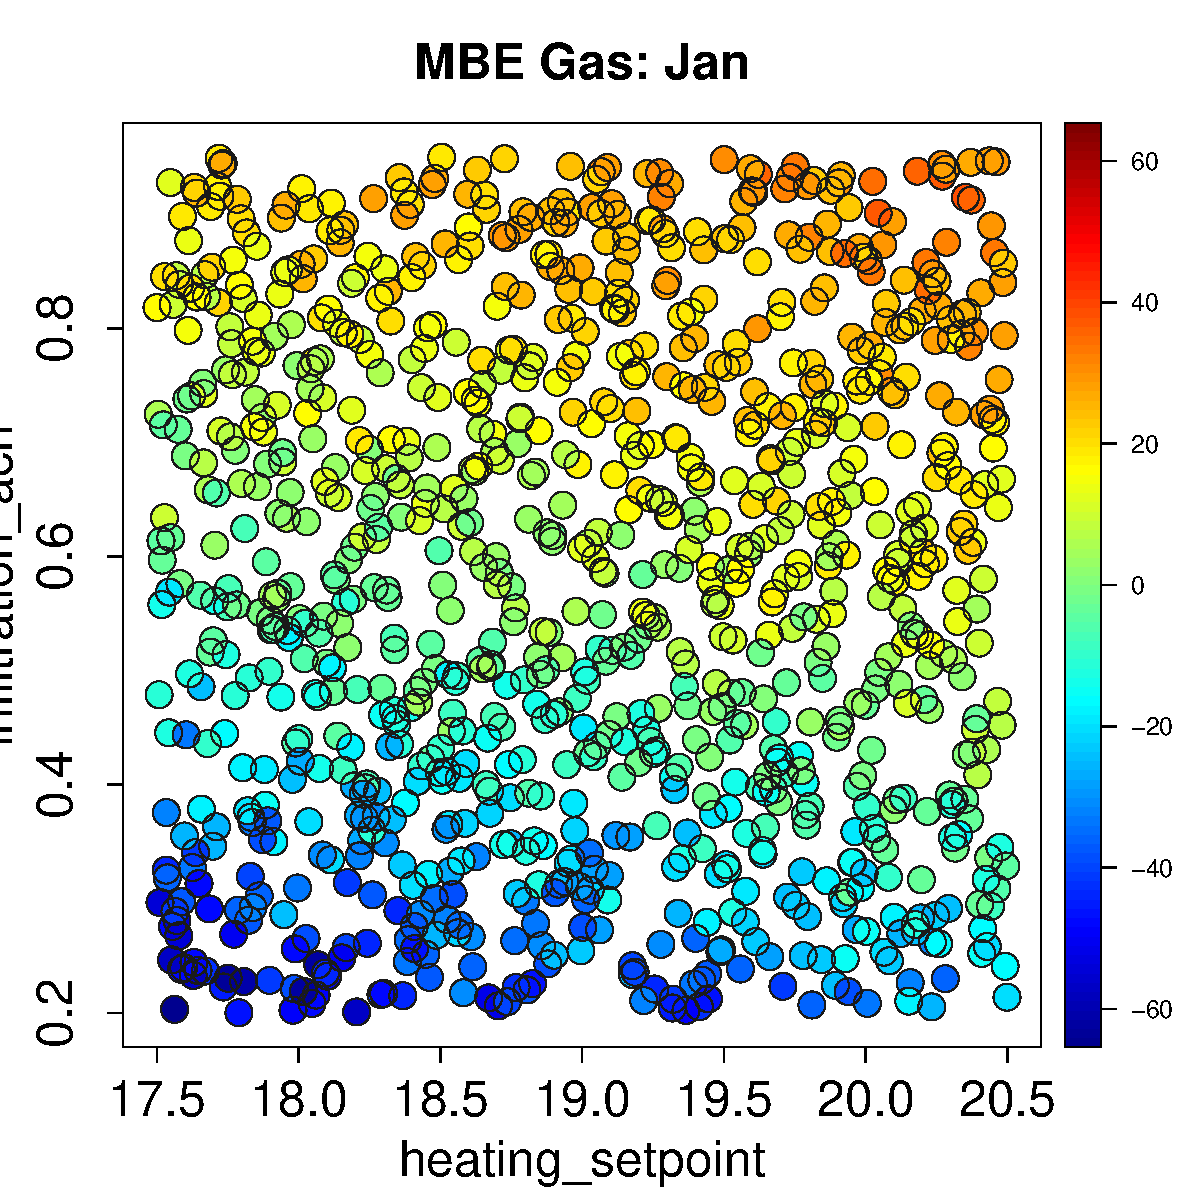
\includegraphics[width=\scale]{MBE/MBE_Gas_01.pdf}
 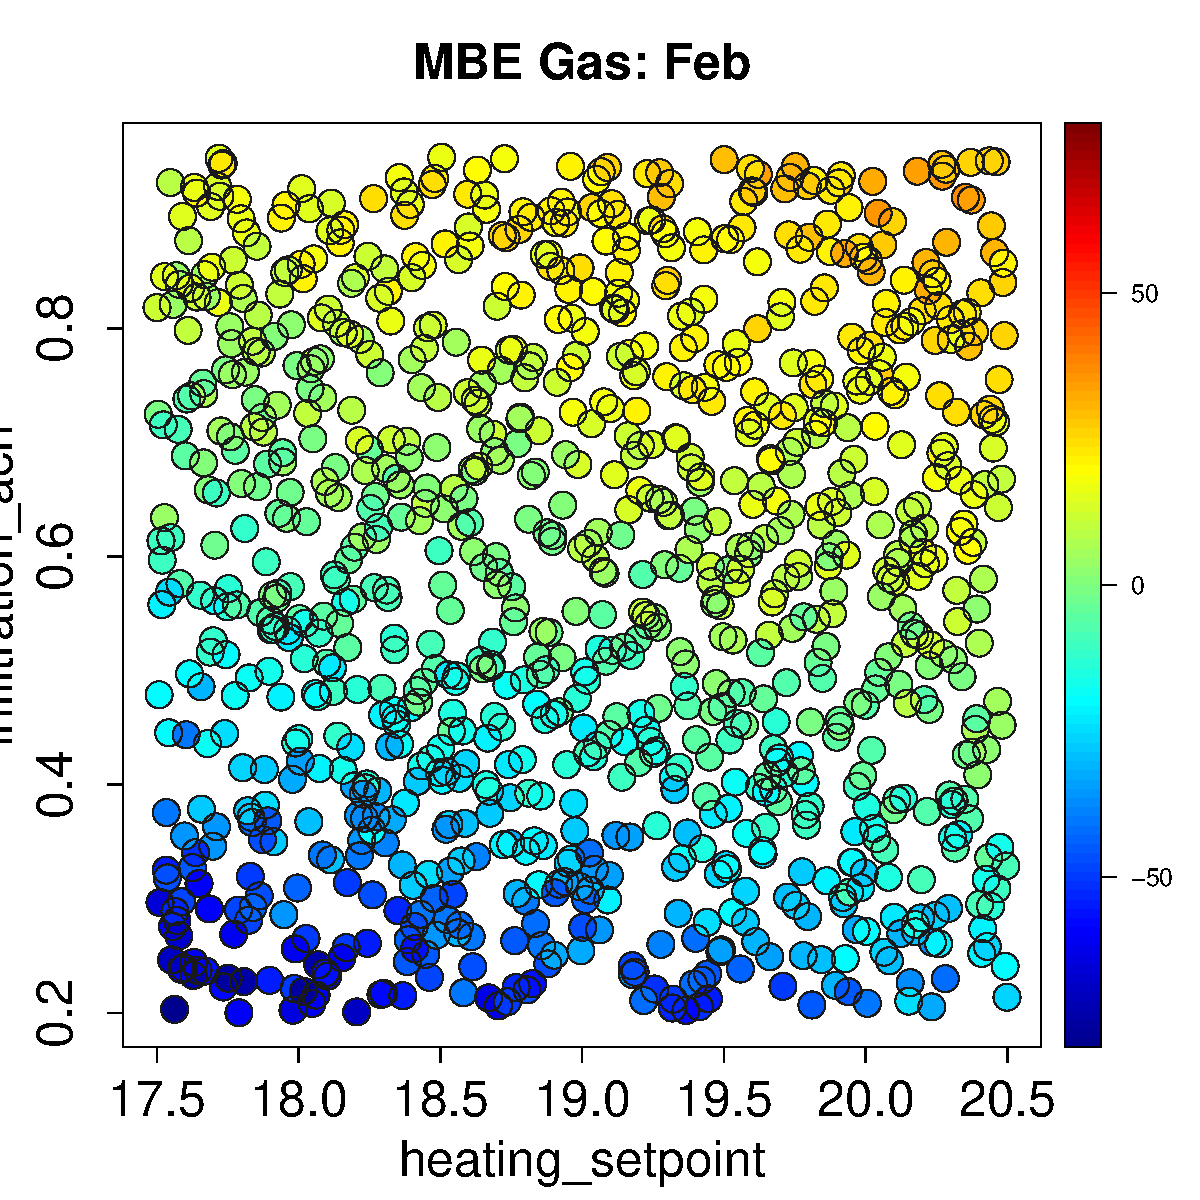
\includegraphics[width=\scale]{MBE/MBE_Gas_02.pdf}
 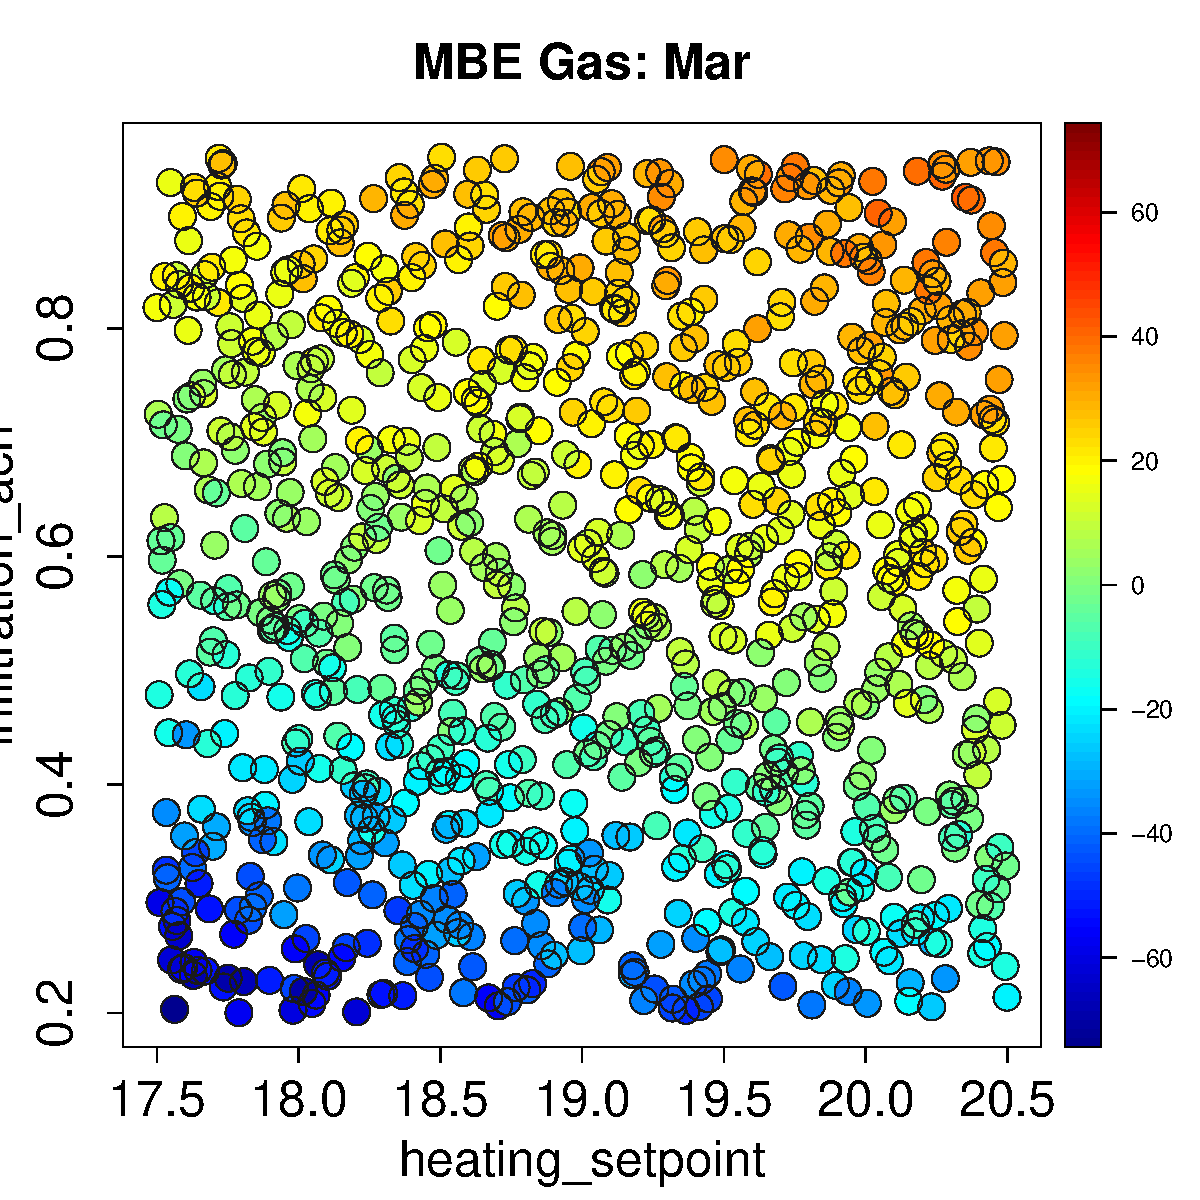
\includegraphics[width=\scale]{MBE/MBE_Gas_03.pdf}\\
 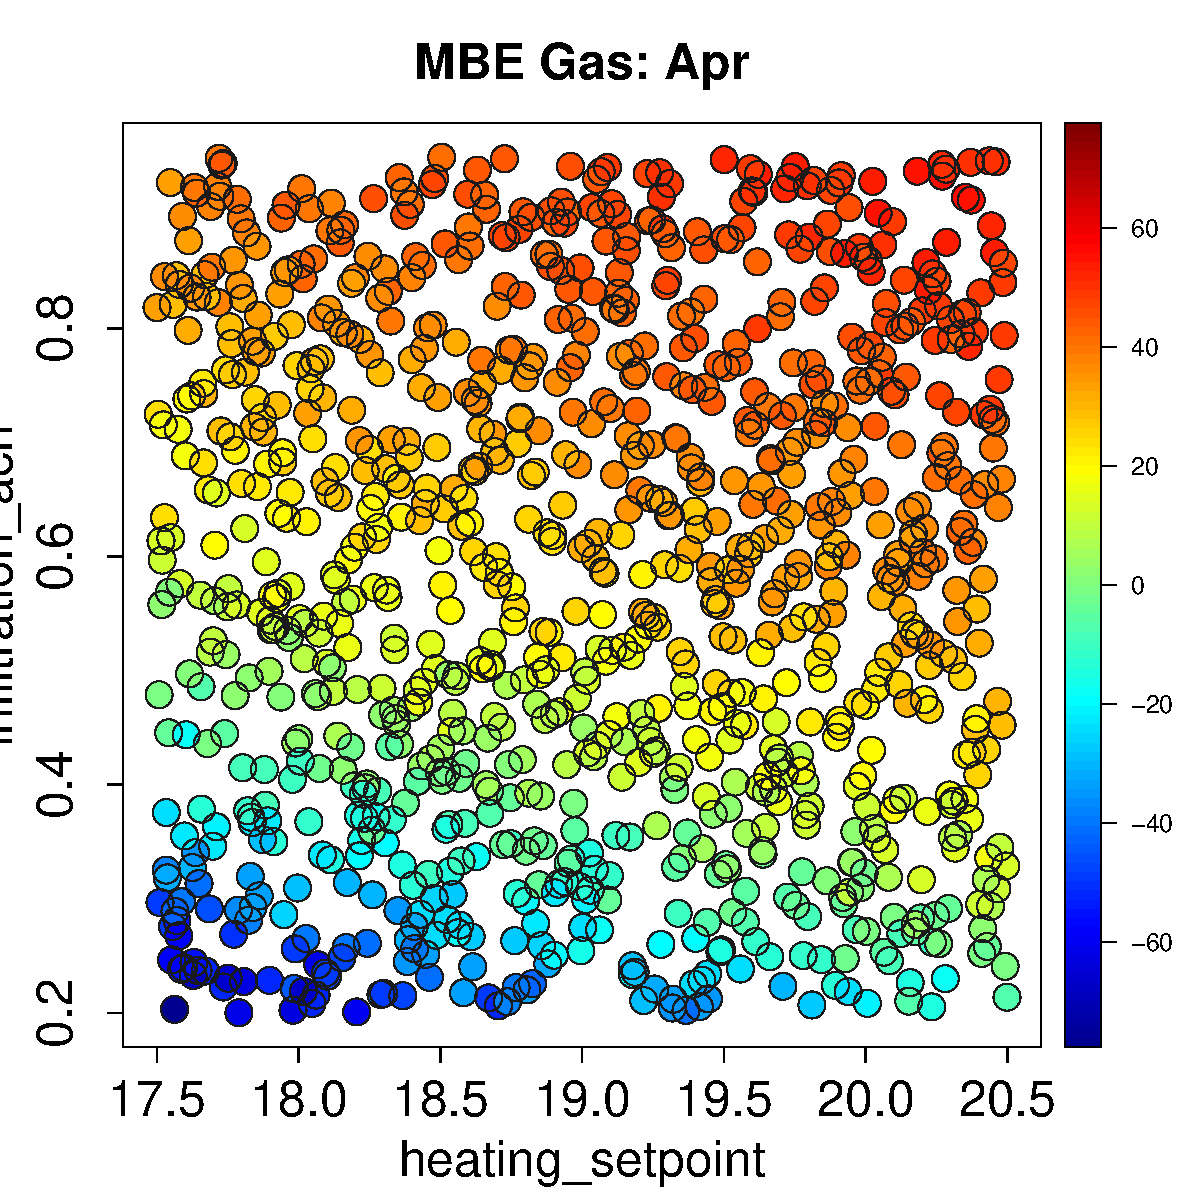
\includegraphics[width=\scale]{MBE/MBE_Gas_04.pdf}
 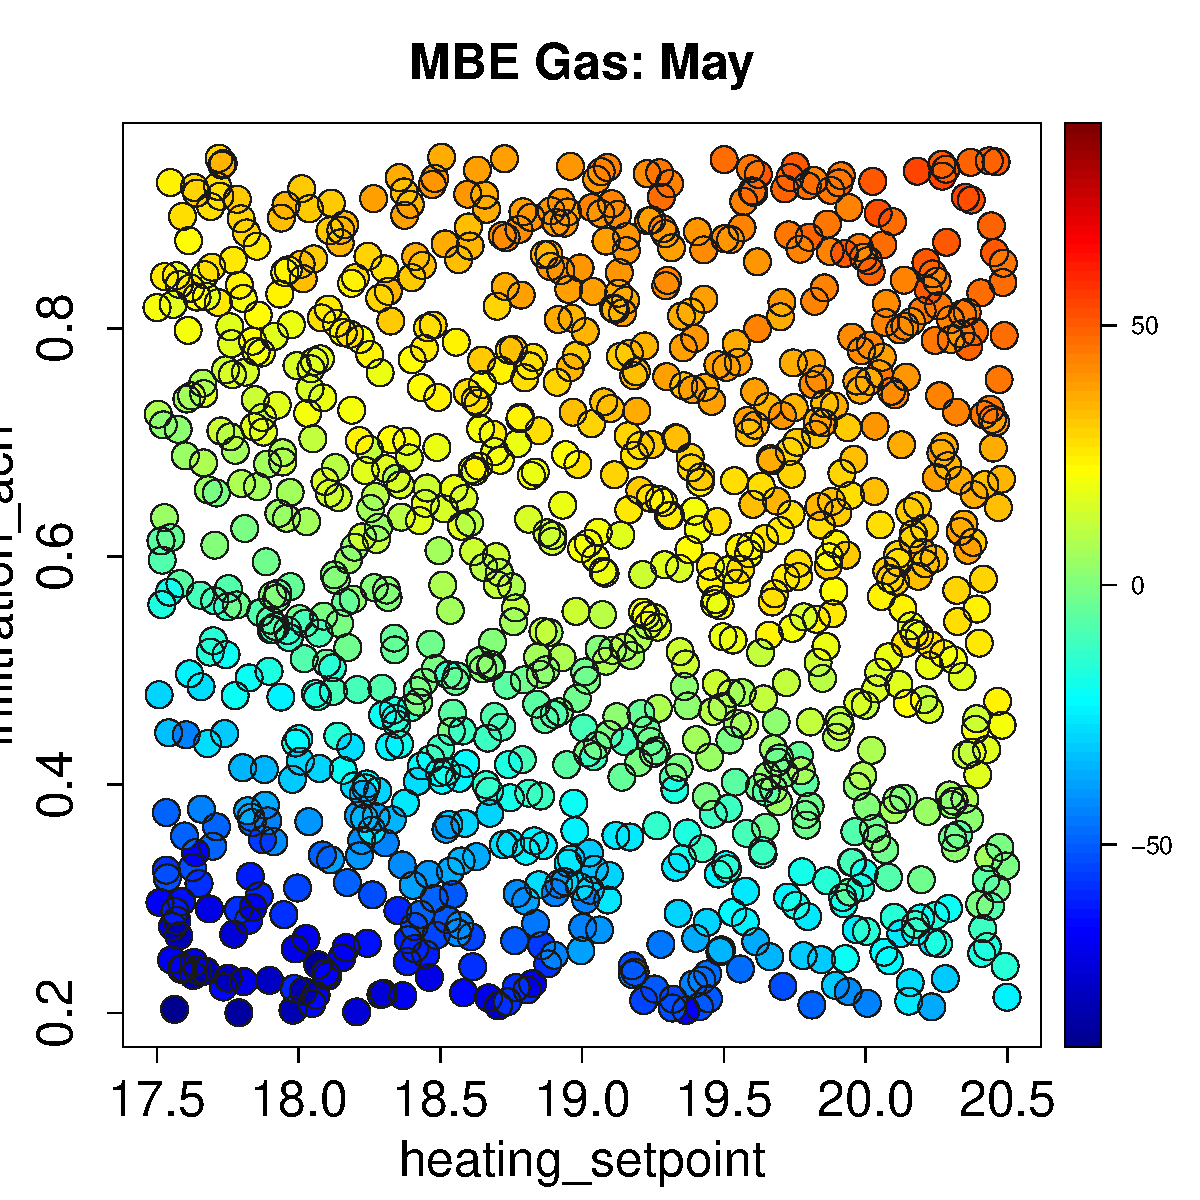
\includegraphics[width=\scale]{MBE/MBE_Gas_05.pdf}
 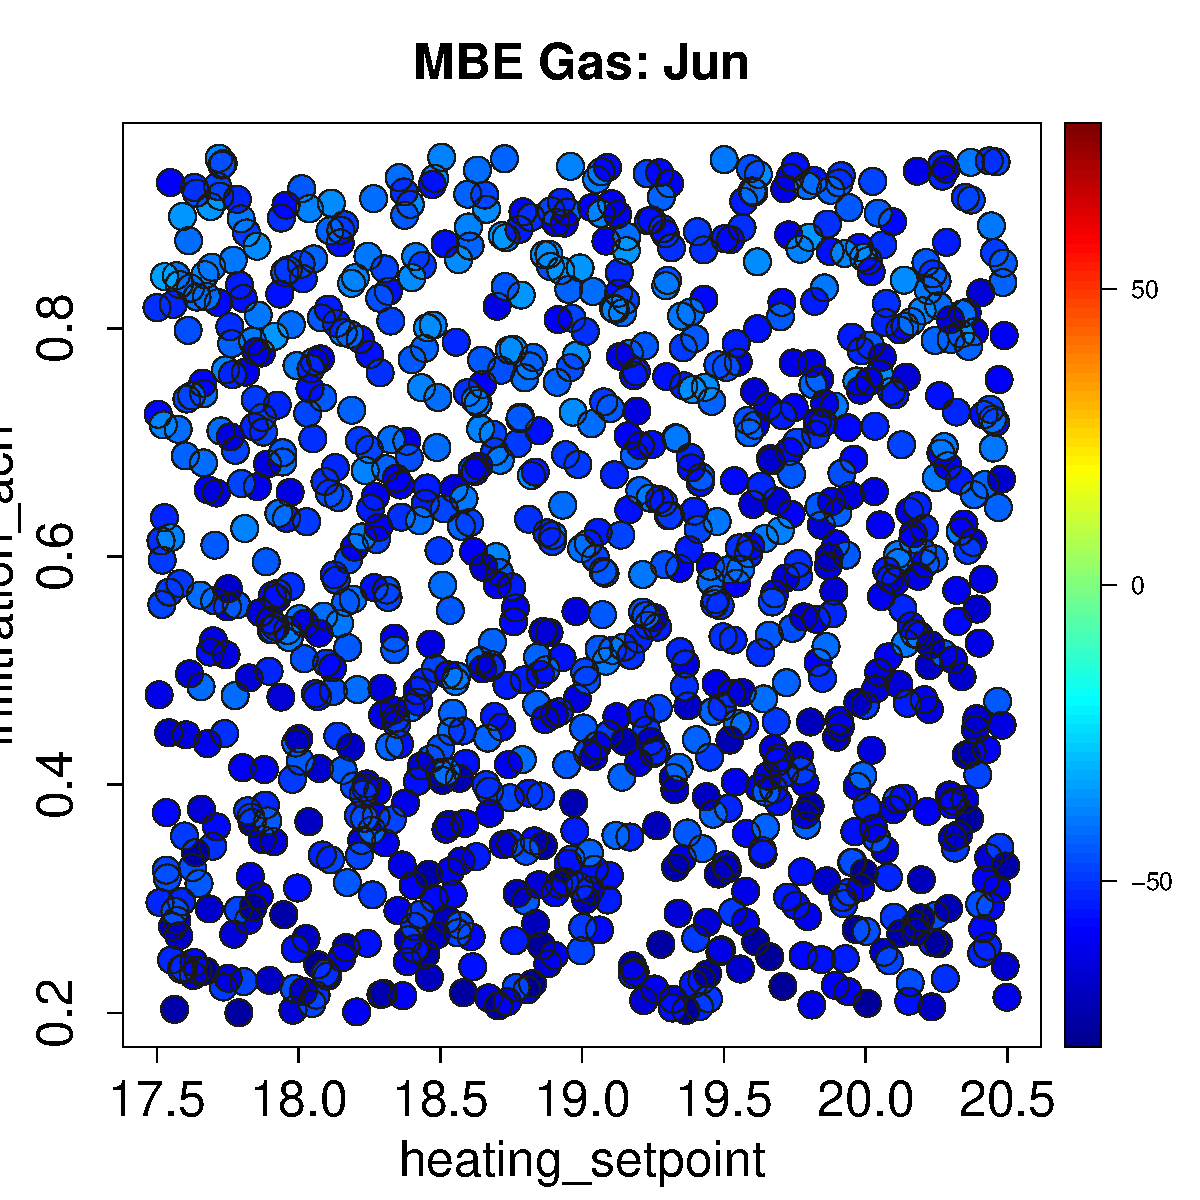
\includegraphics[width=\scale]{MBE/MBE_Gas_06.pdf}\\
 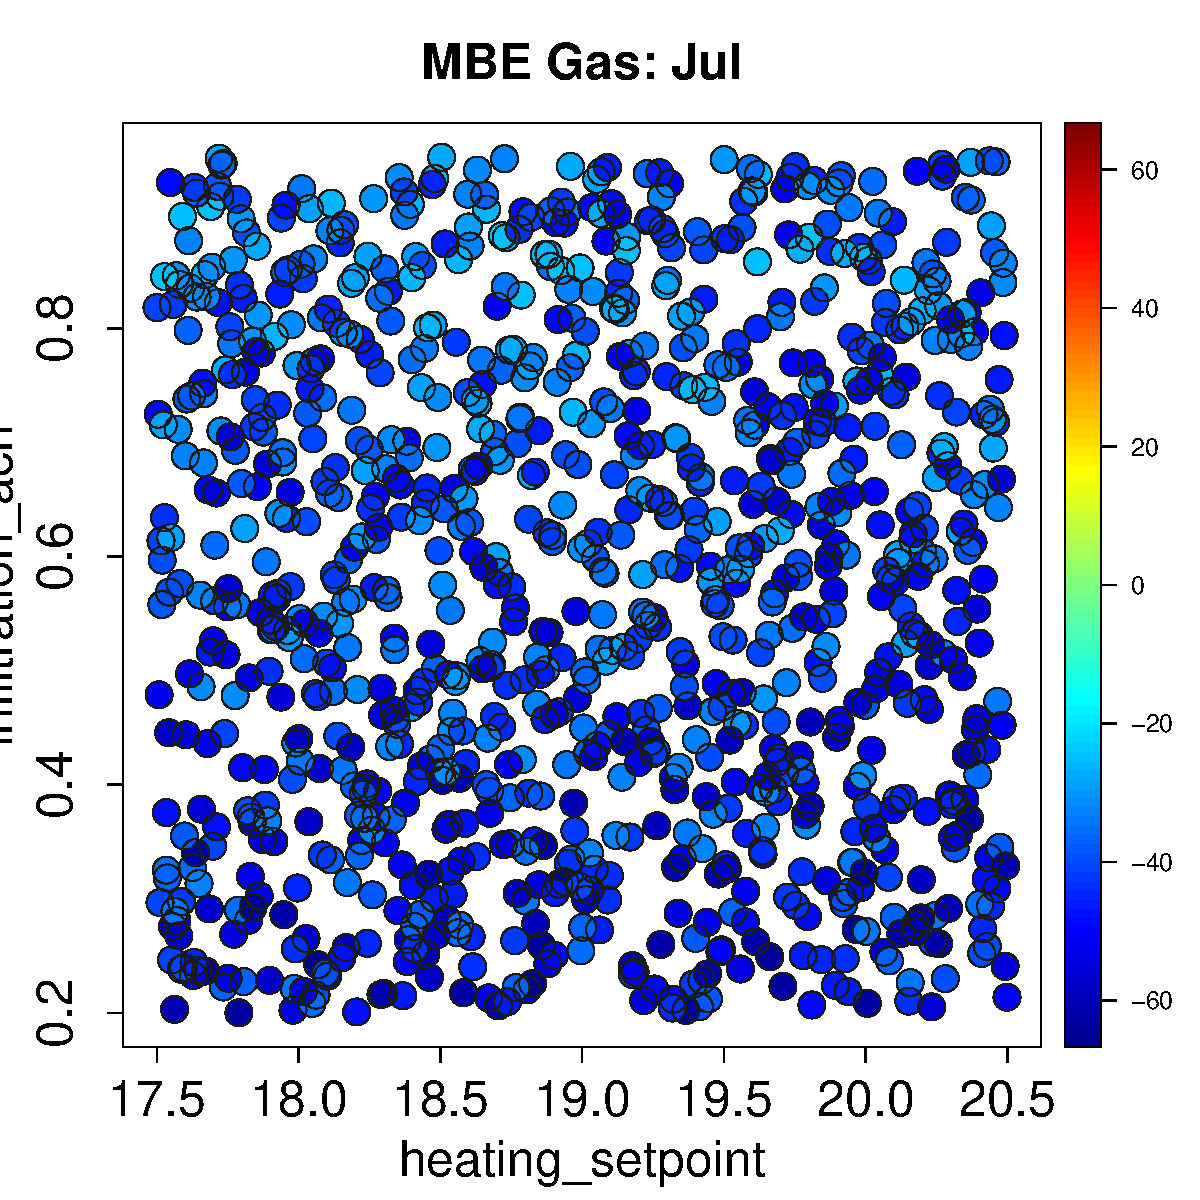
\includegraphics[width=\scale]{MBE/MBE_Gas_07.pdf}
 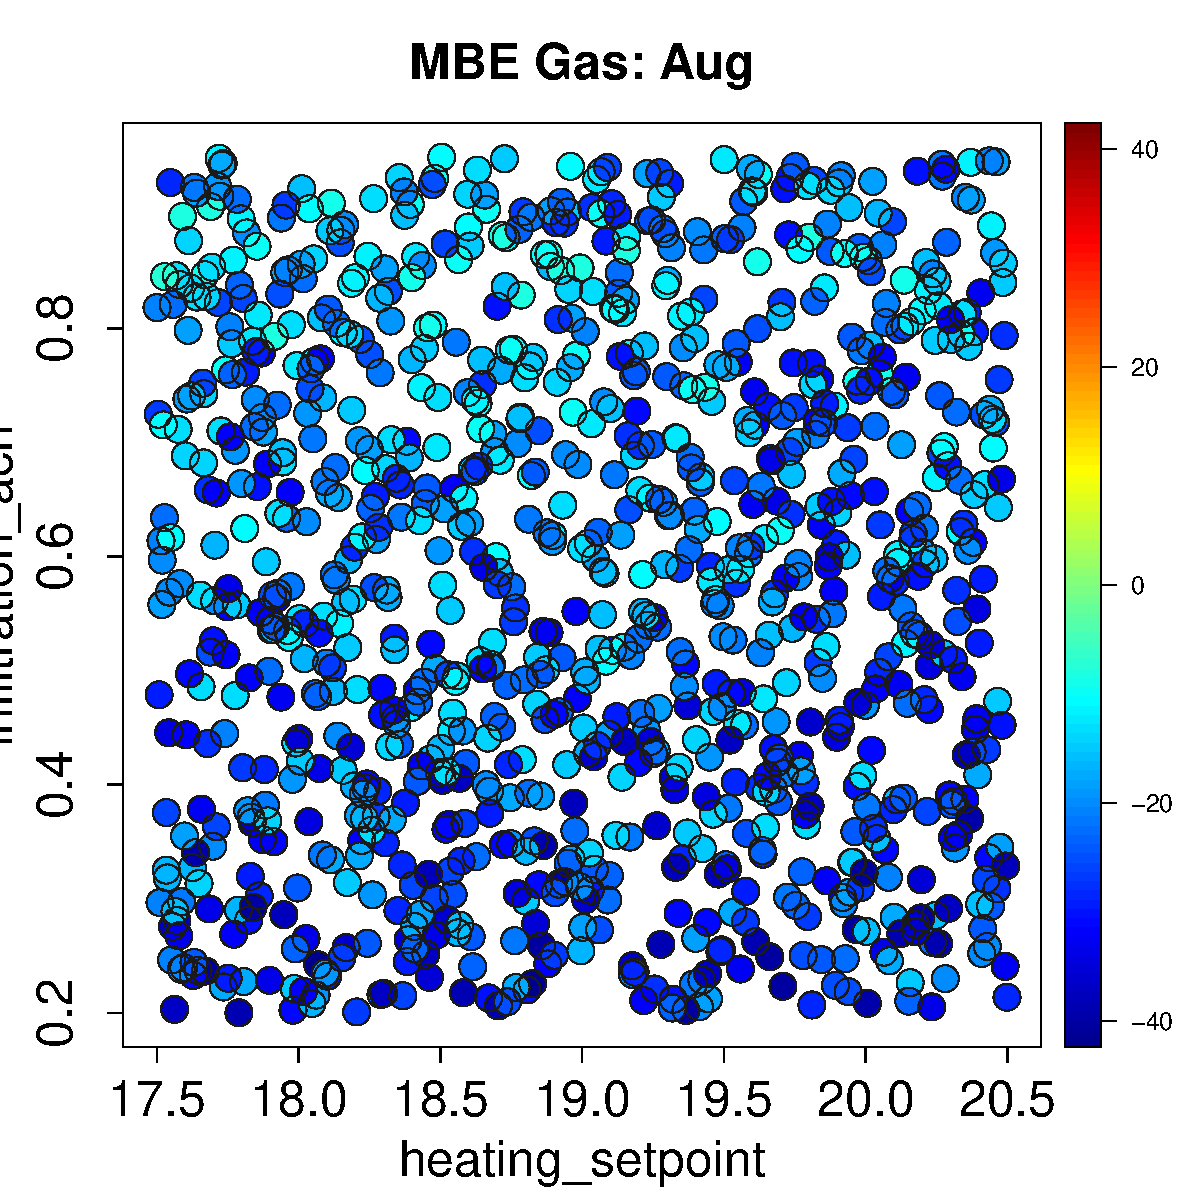
\includegraphics[width=\scale]{MBE/MBE_Gas_08.pdf}
 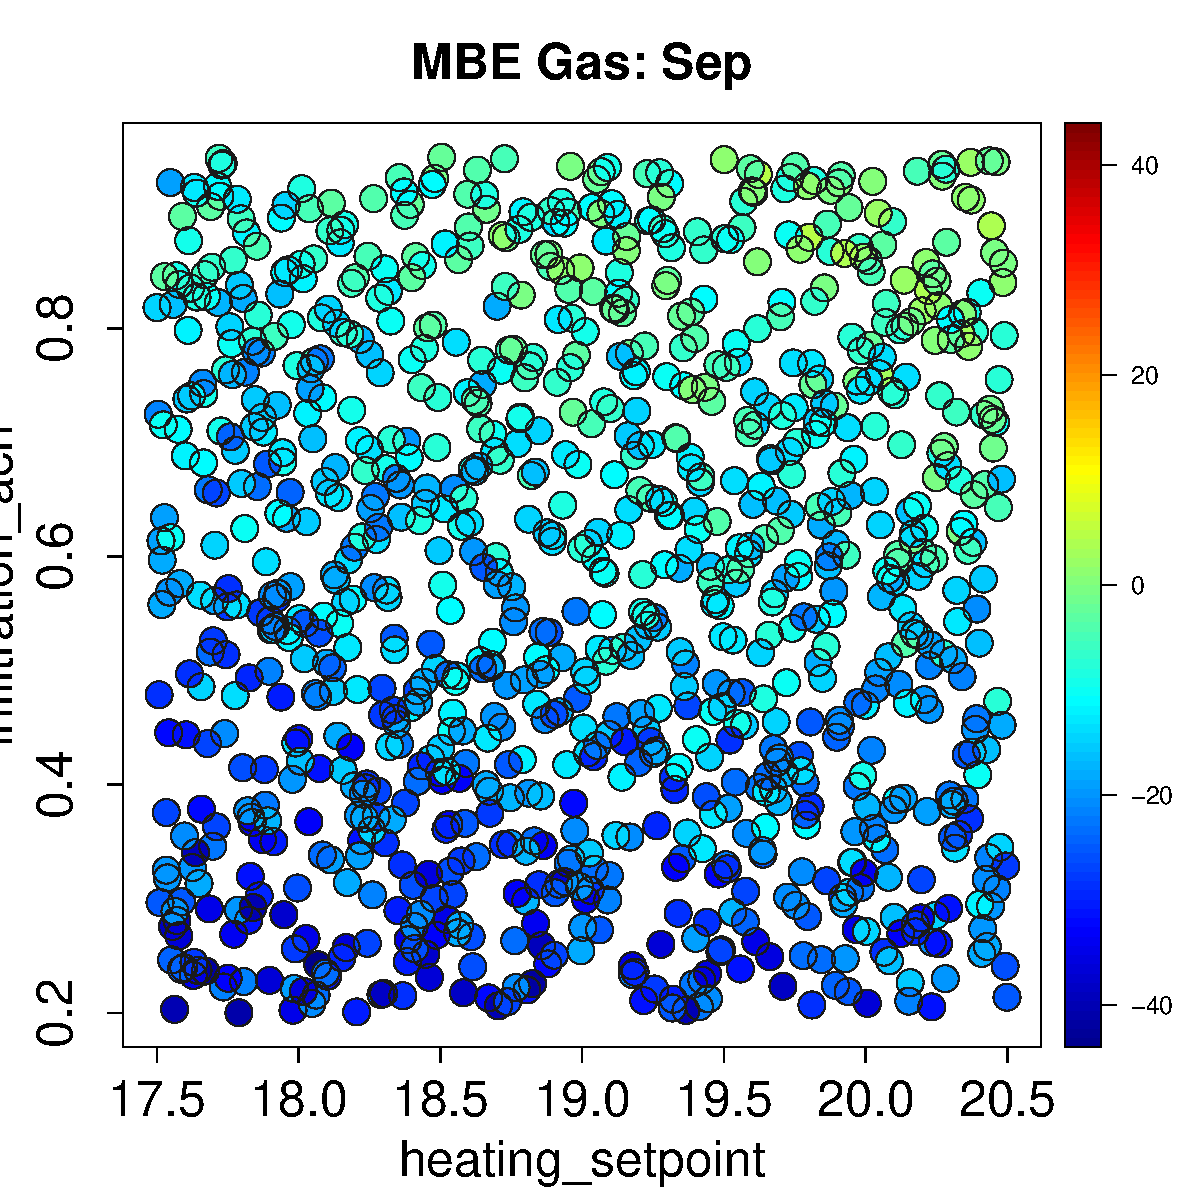
\includegraphics[width=\scale]{MBE/MBE_Gas_09.pdf}\\
 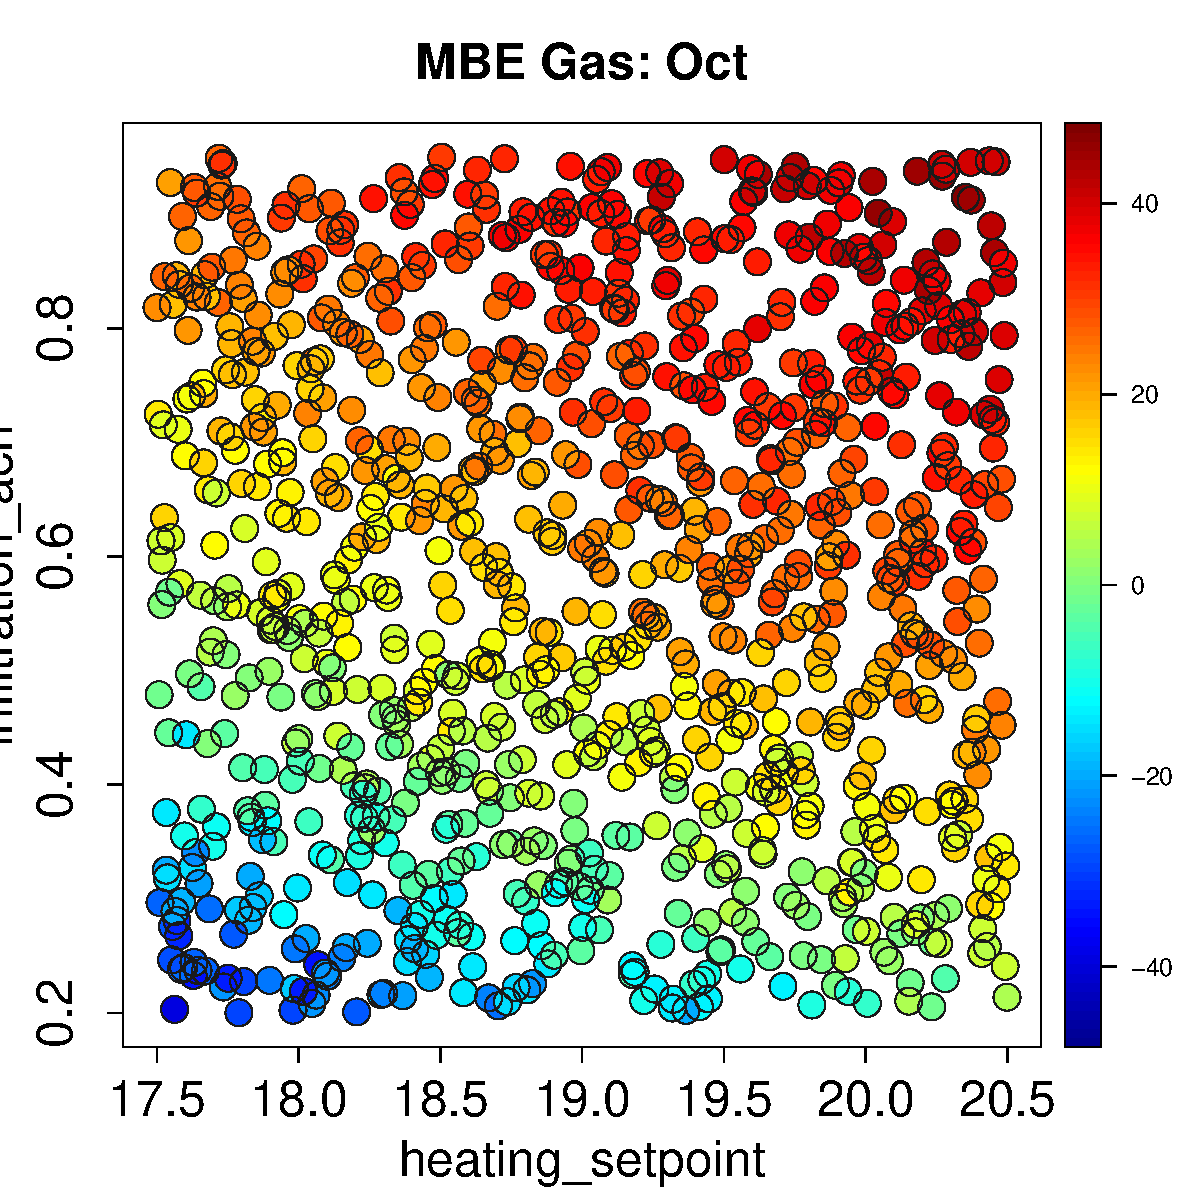
\includegraphics[width=\scale]{MBE/MBE_Gas_10.pdf}
 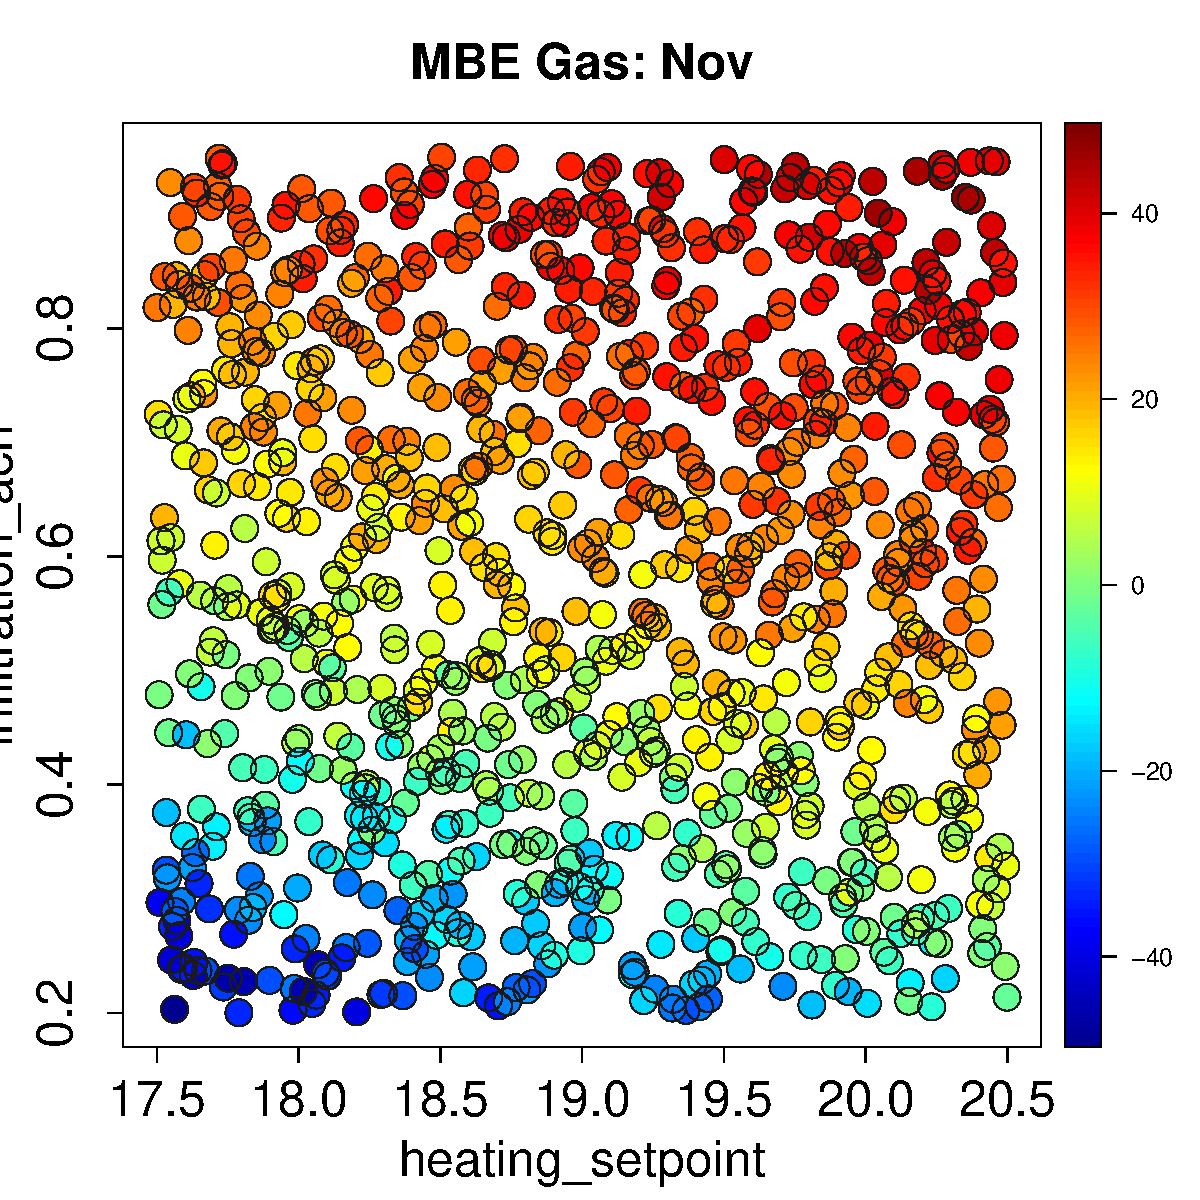
\includegraphics[width=\scale]{MBE/MBE_Gas_11.pdf}
 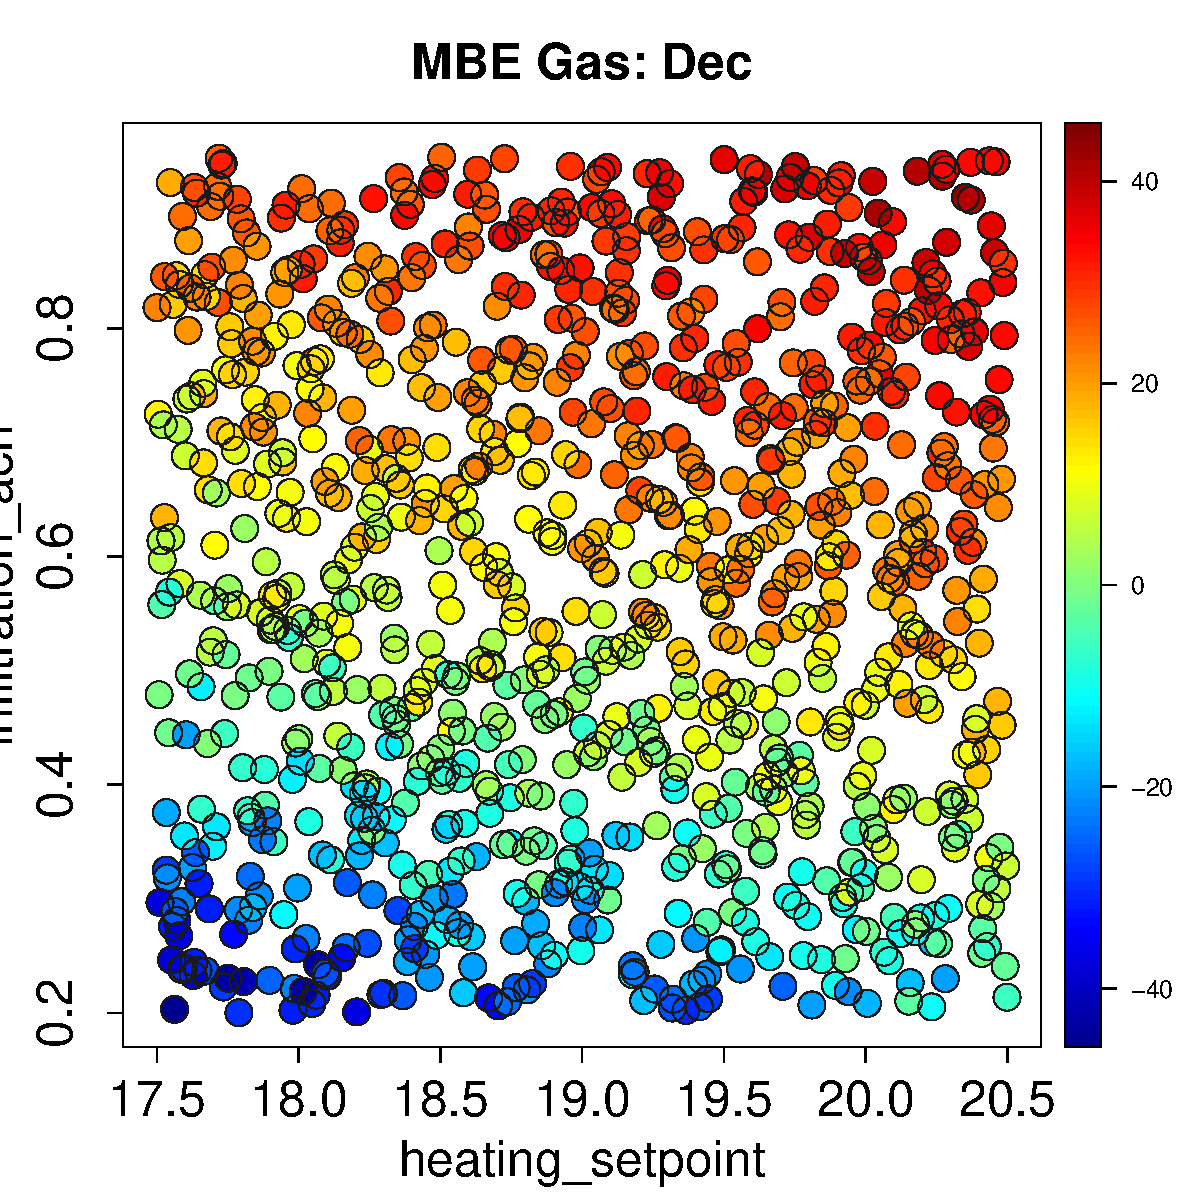
\includegraphics[width=\scale]{MBE/MBE_Gas_12.pdf}\\
 \caption{Scatter plots of the first (heating setpoint) and sixth (infiltration rate) coordinates of the 1000 simulations. The color represents the value, in percentage, of the MBE for each such simulation, and for the 12 months. ASHRAE guidelines suggest to consider as ``plausible'' runs for which $-5\% \leq \text{MBE} \leq 5\%$.}
 \label{Fig_Output_Hist}
\end{figure}





\renewcommand{\scale}{12.2em}
\begin{figure}
\centering
 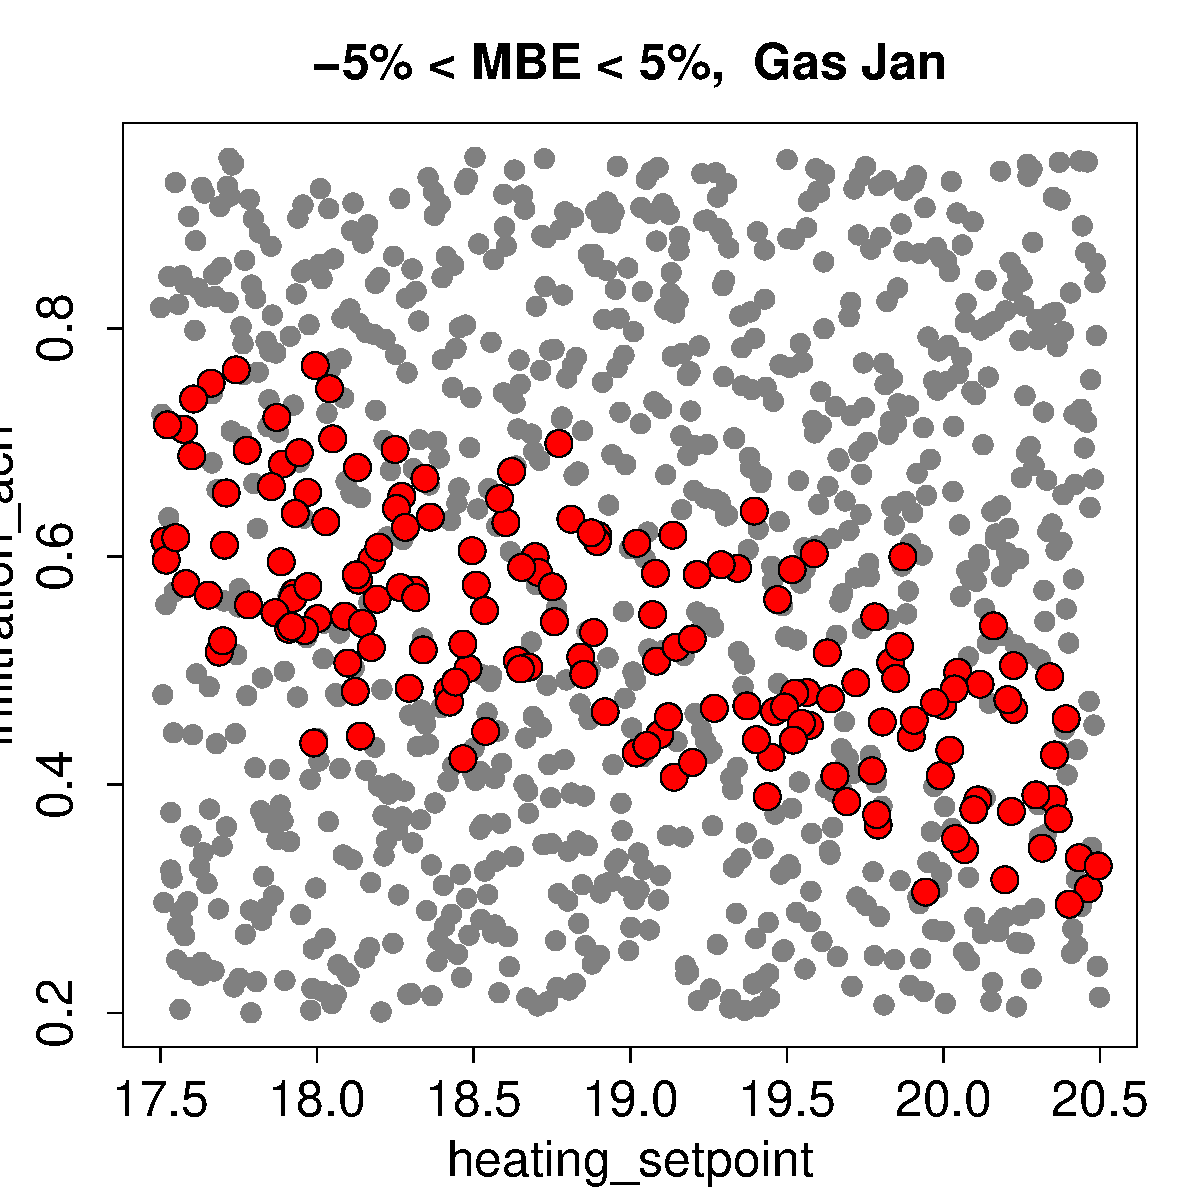
\includegraphics[width=\scale]{MBE/SelectedMBE_Gas_01.pdf}
 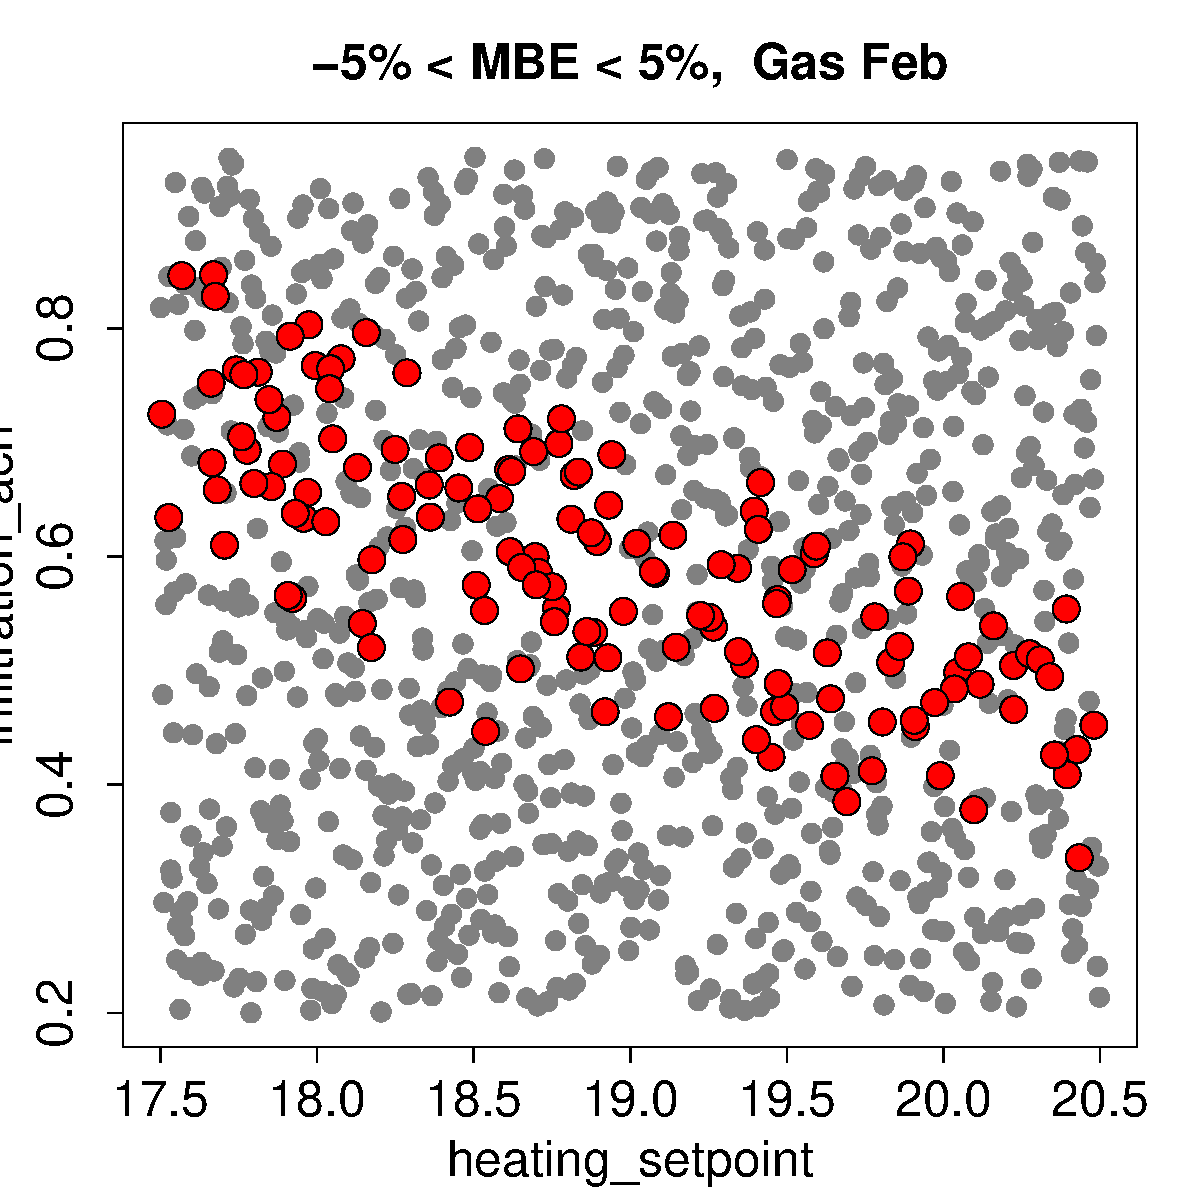
\includegraphics[width=\scale]{MBE/SelectedMBE_Gas_02.pdf}
 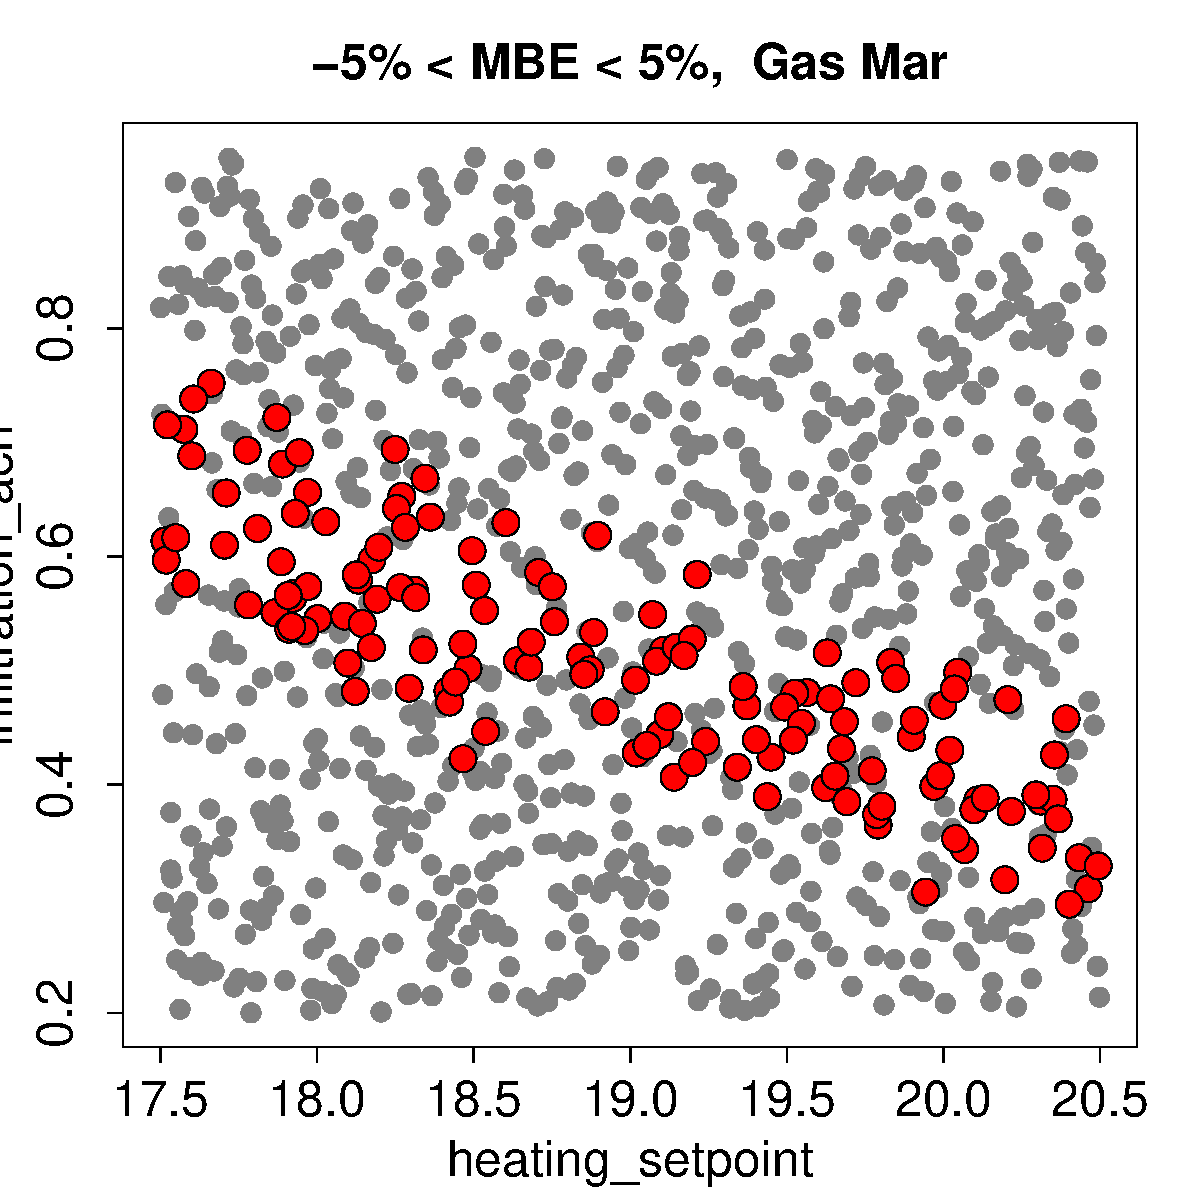
\includegraphics[width=\scale]{MBE/SelectedMBE_Gas_03.pdf}\\
 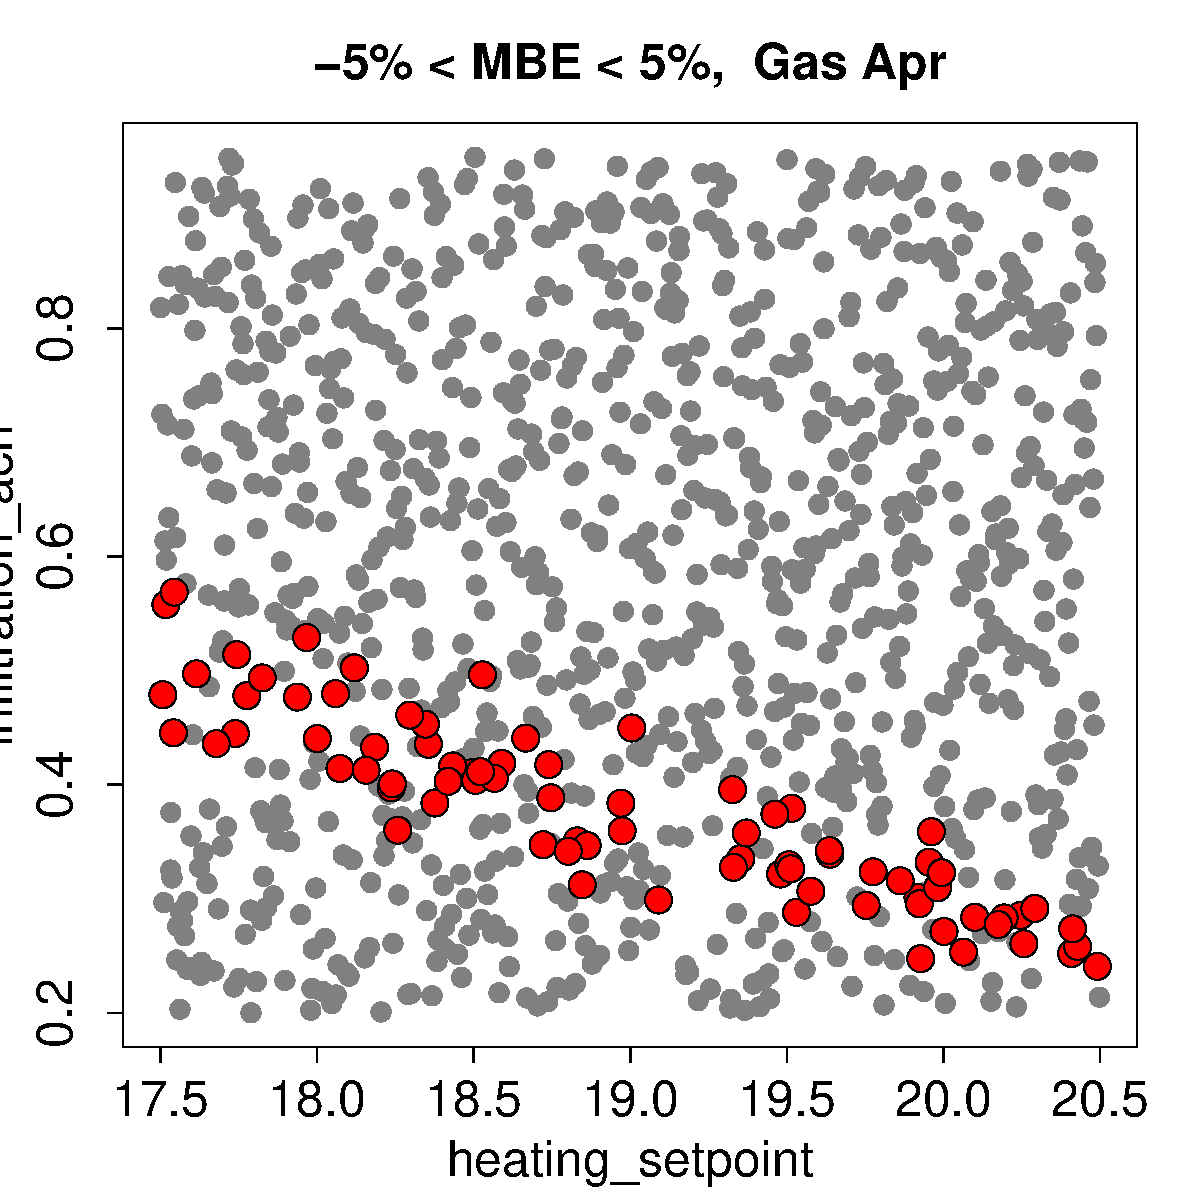
\includegraphics[width=\scale]{MBE/SelectedMBE_Gas_04.pdf}
 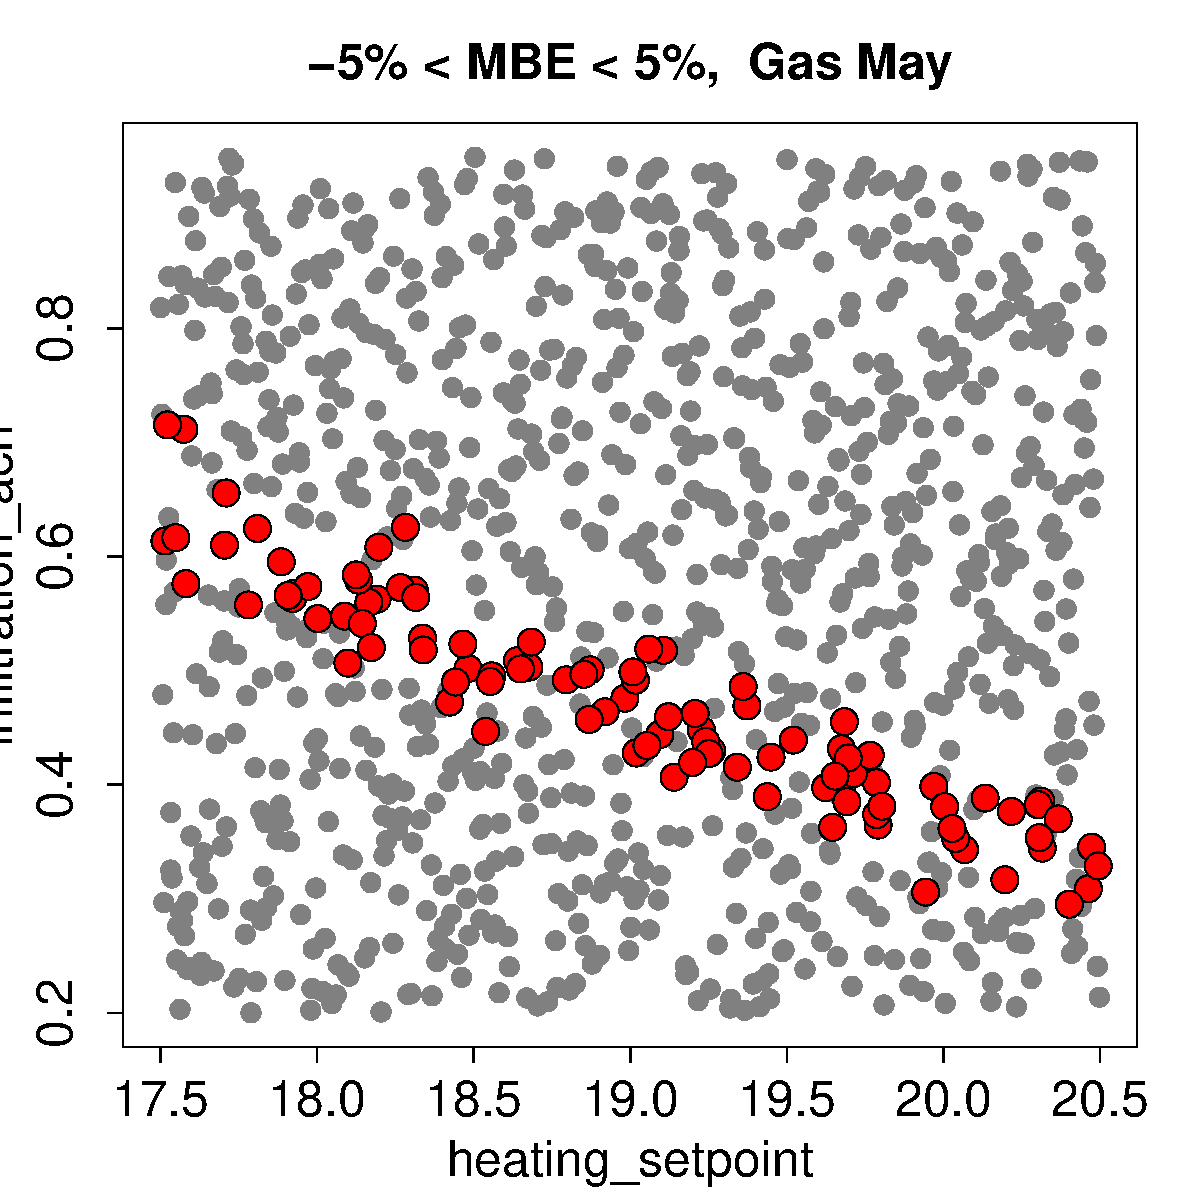
\includegraphics[width=\scale]{MBE/SelectedMBE_Gas_05.pdf}
 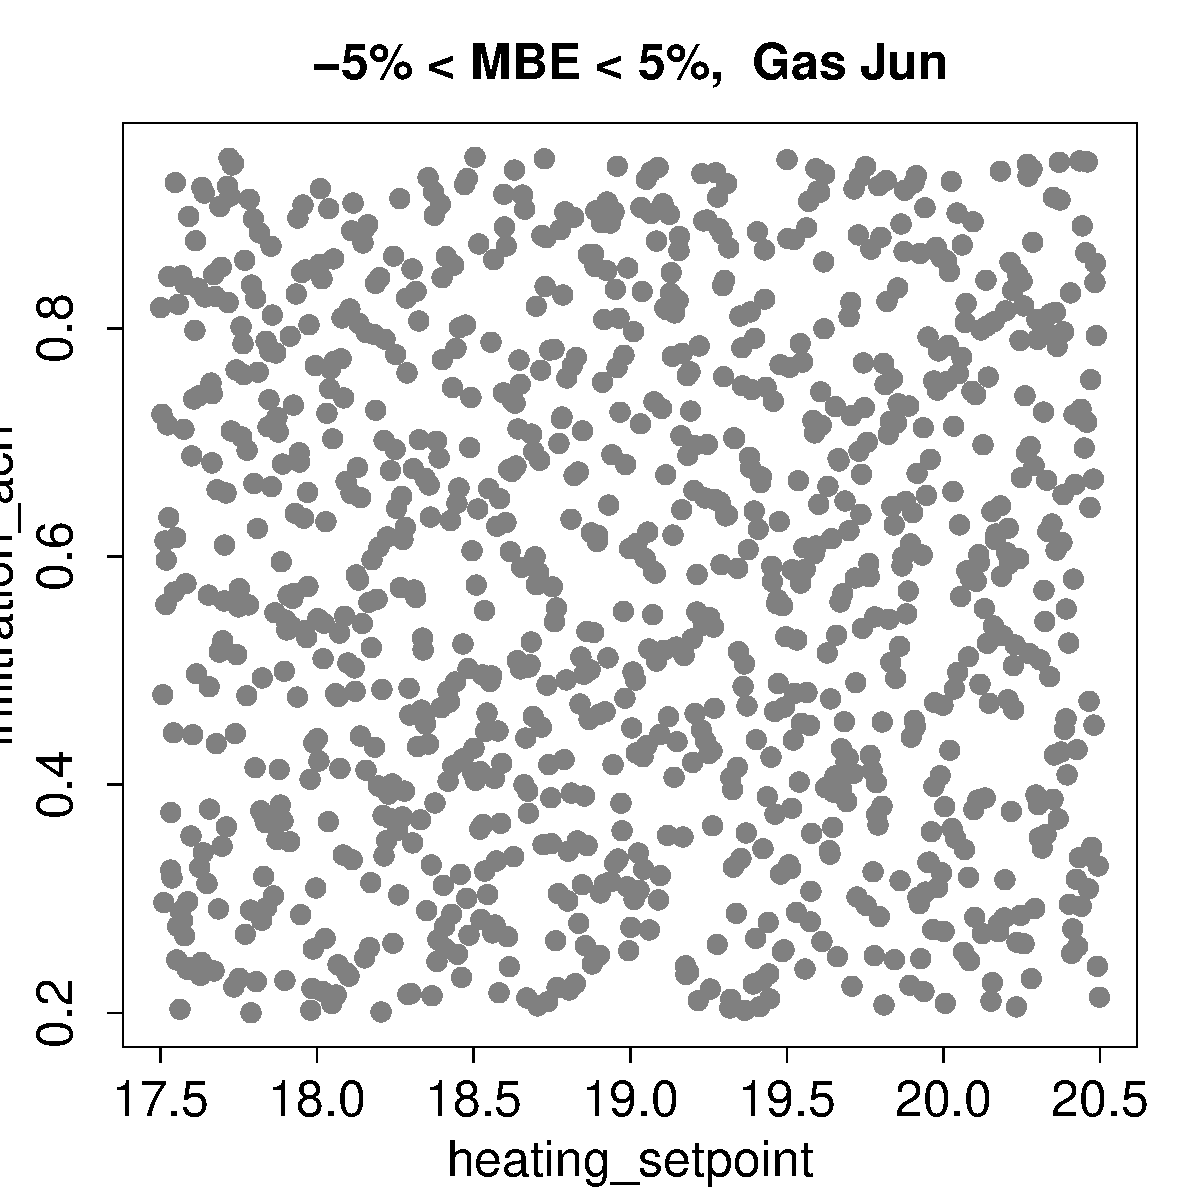
\includegraphics[width=\scale]{MBE/SelectedMBE_Gas_06.pdf}\\
 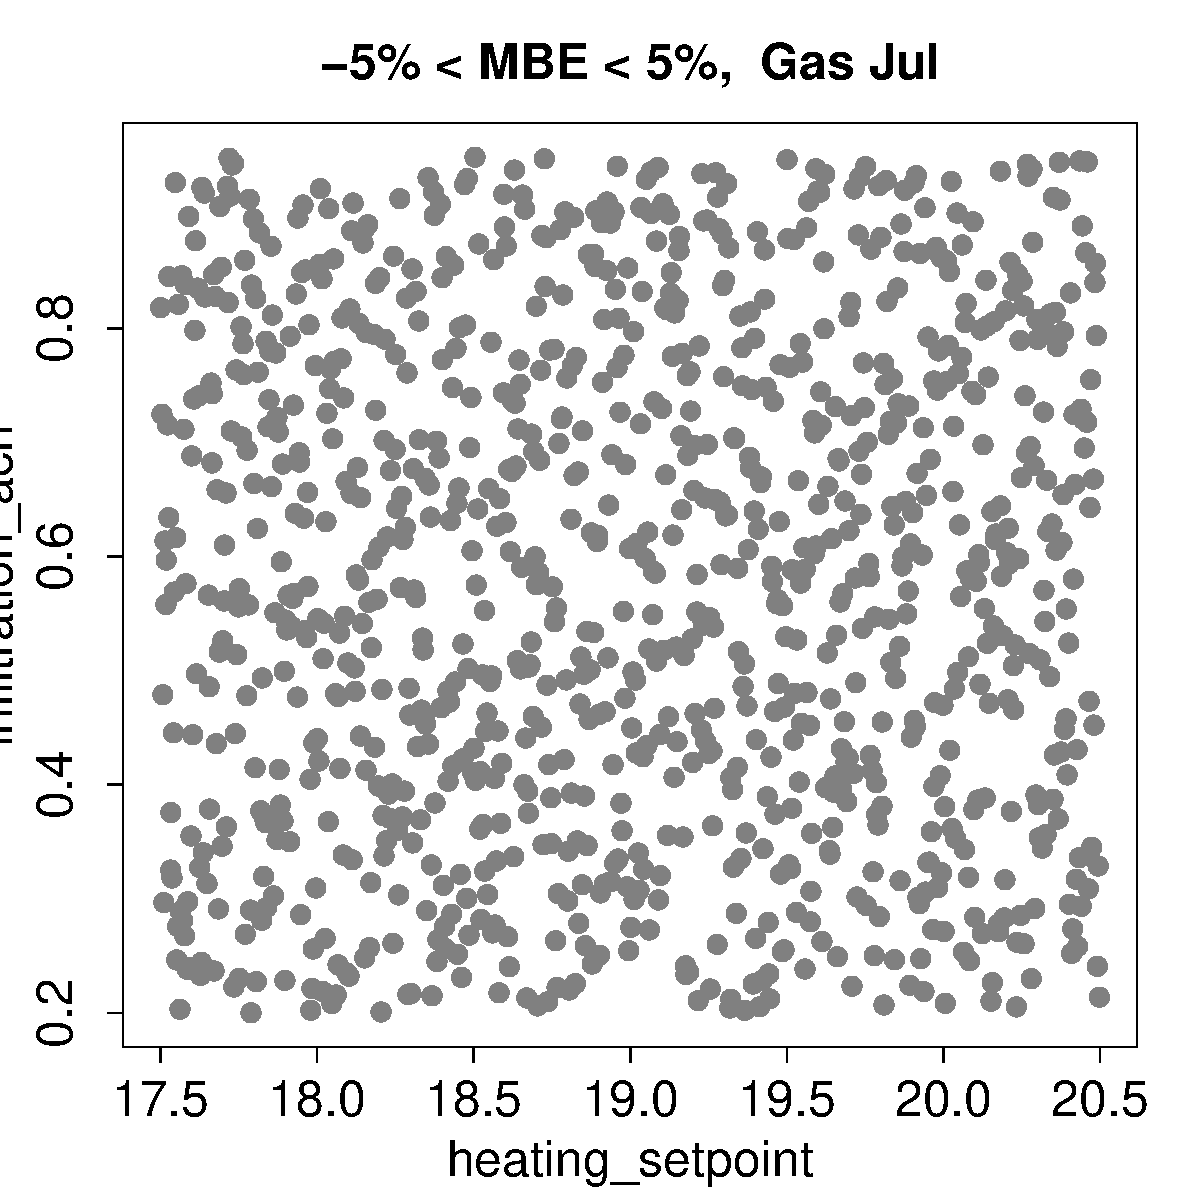
\includegraphics[width=\scale]{MBE/SelectedMBE_Gas_07.pdf}
 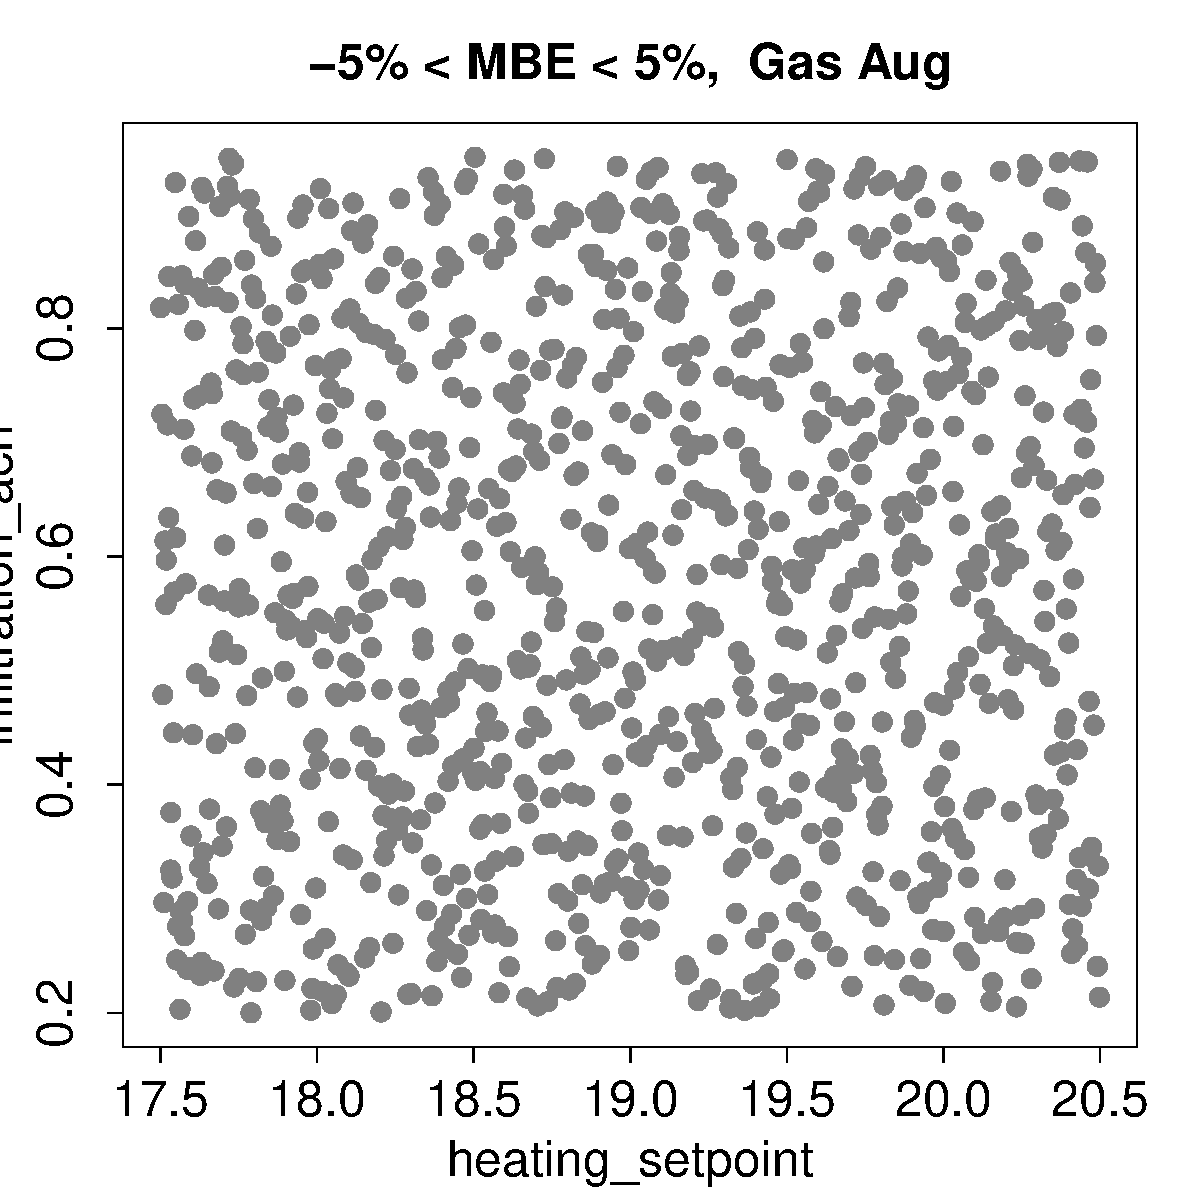
\includegraphics[width=\scale]{MBE/SelectedMBE_Gas_08.pdf}
 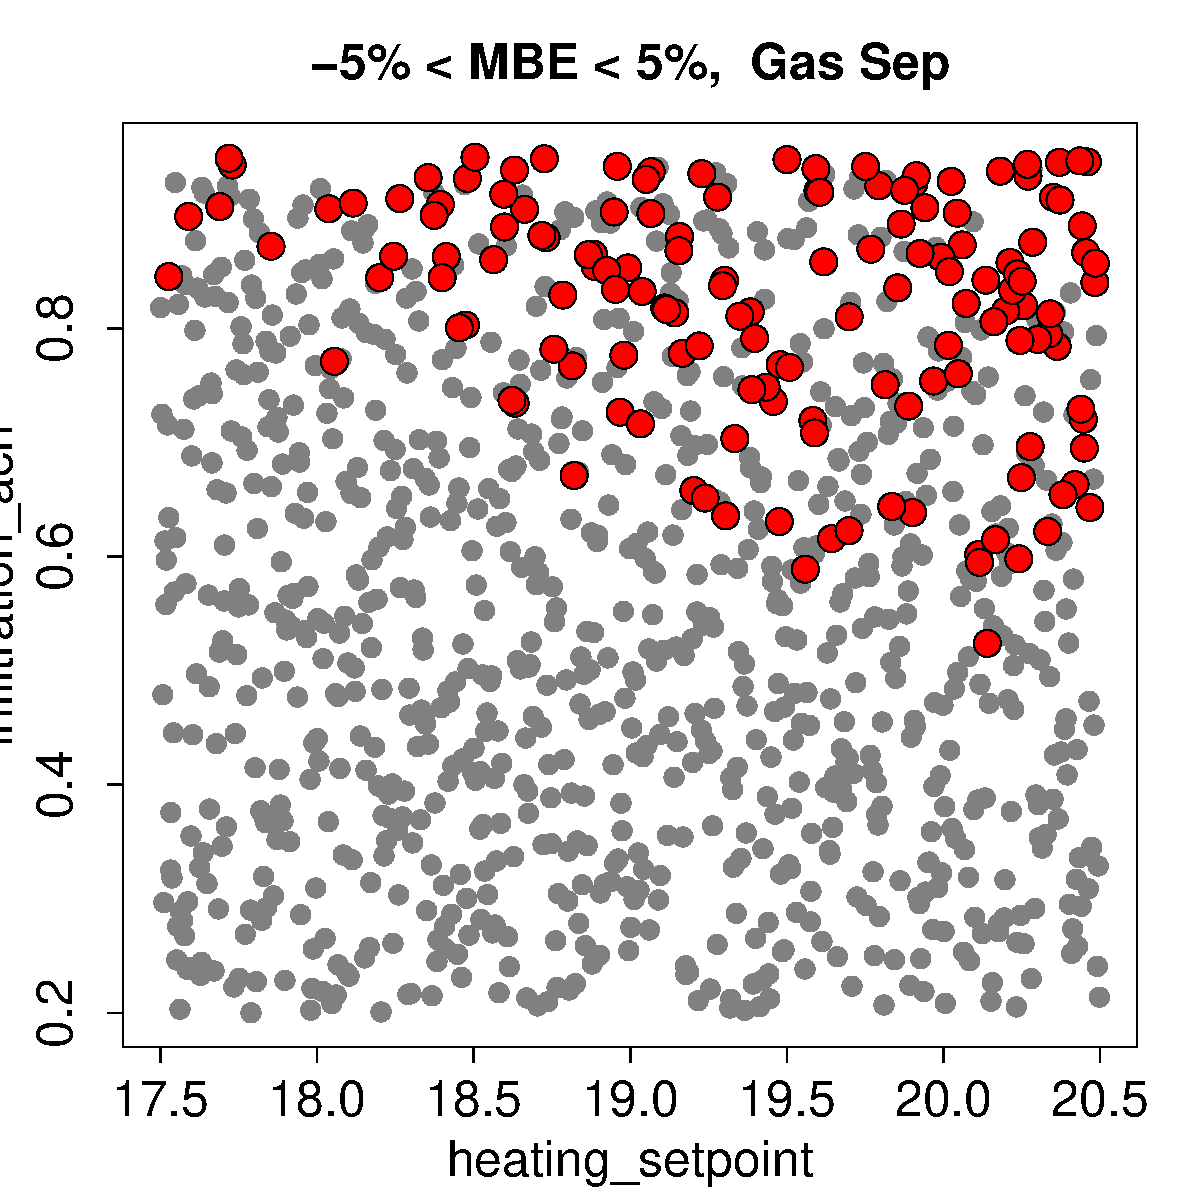
\includegraphics[width=\scale]{MBE/SelectedMBE_Gas_09.pdf}\\
 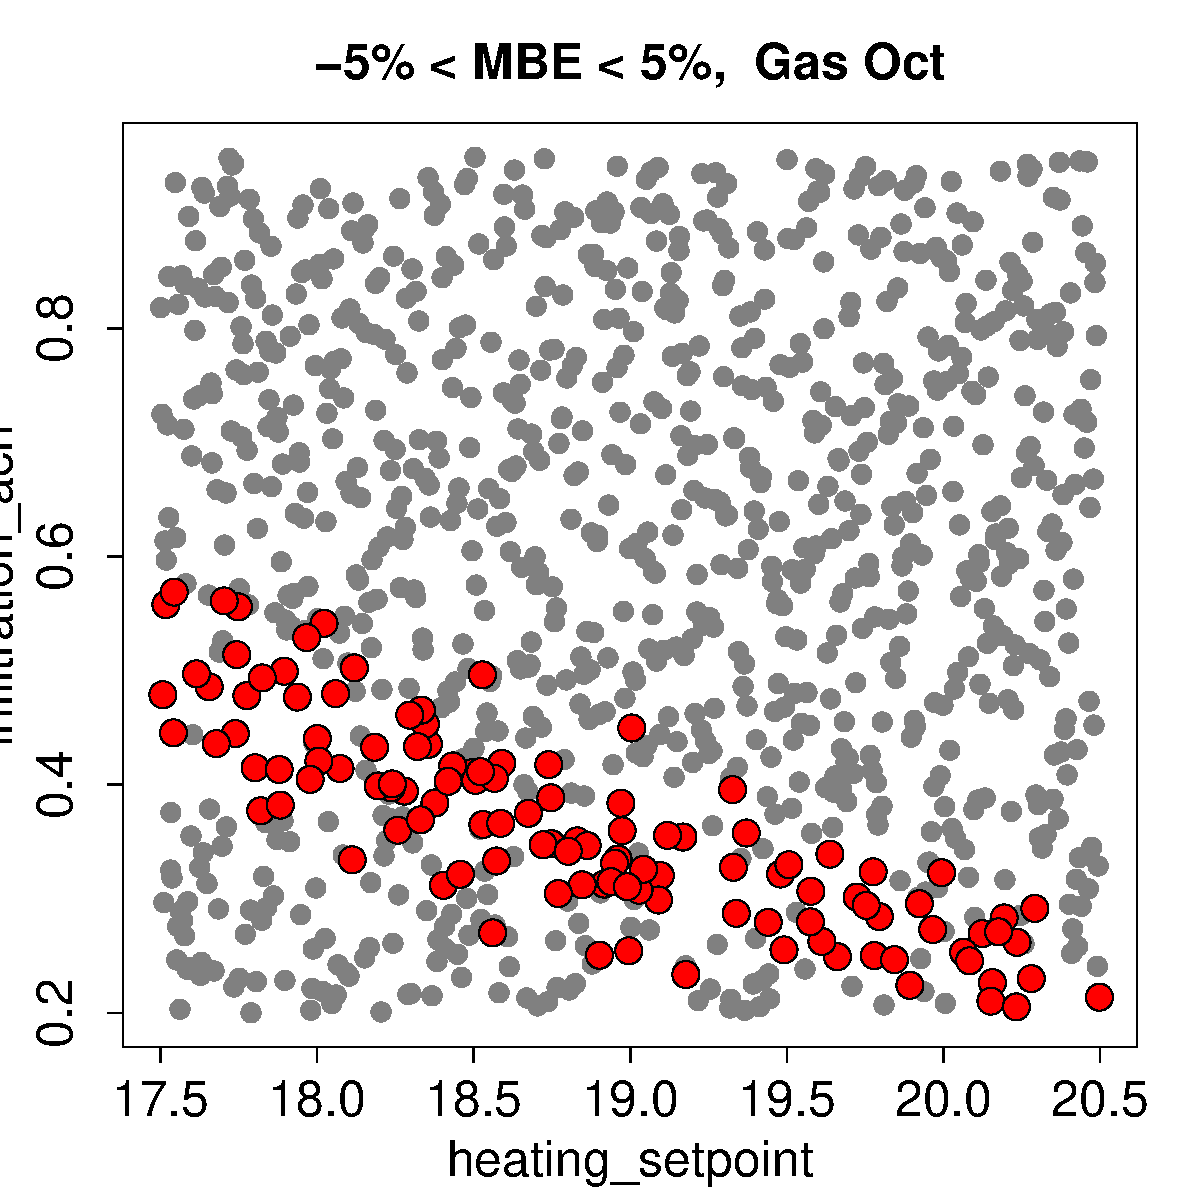
\includegraphics[width=\scale]{MBE/SelectedMBE_Gas_10.pdf}
 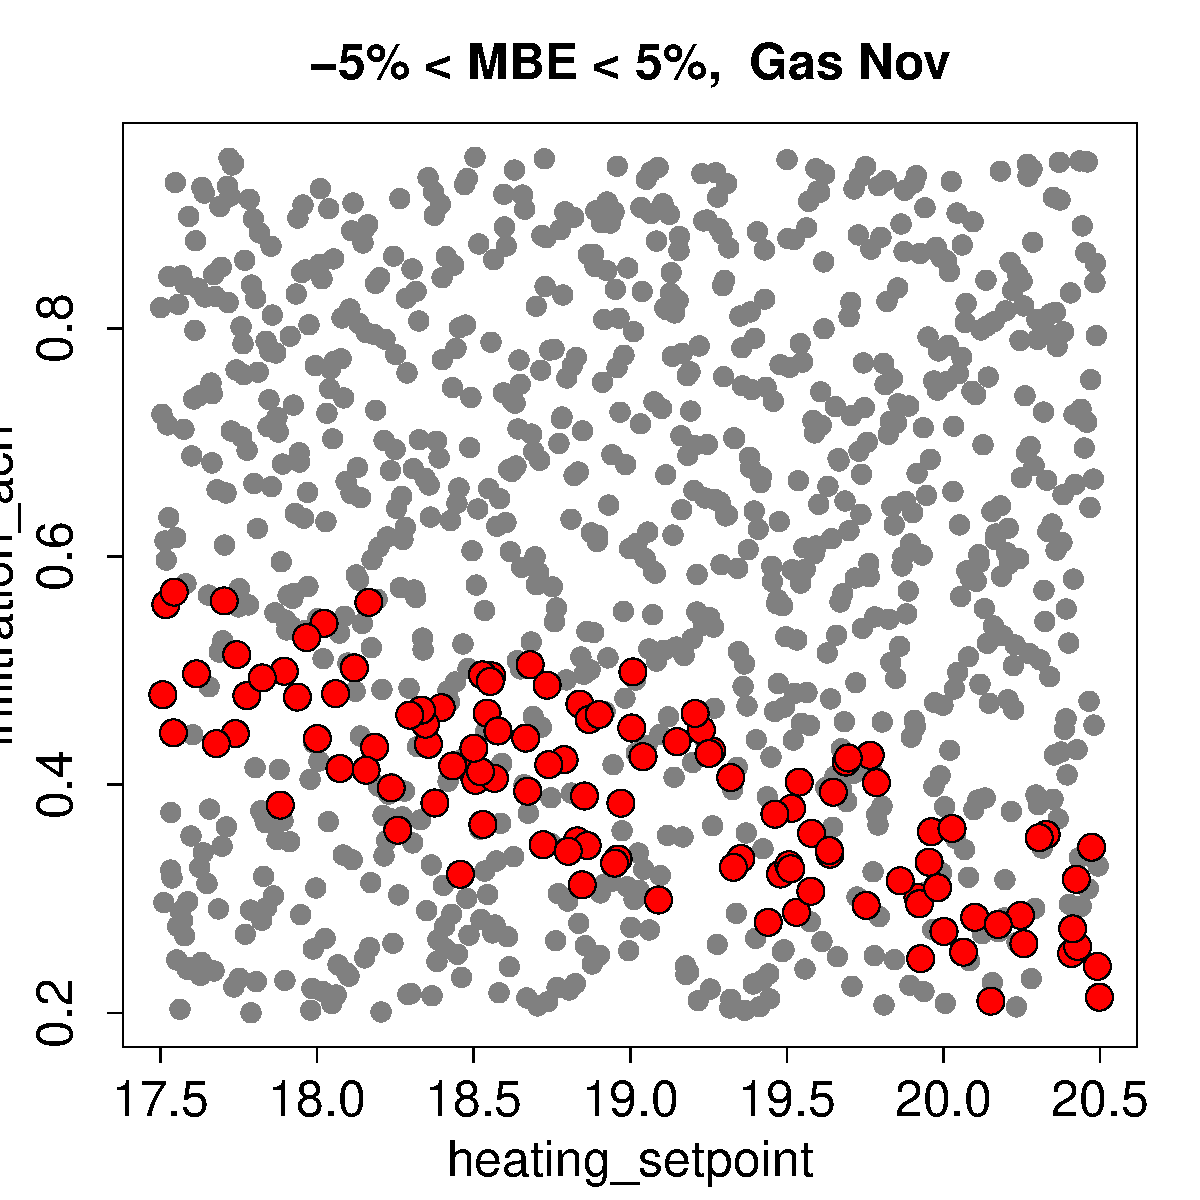
\includegraphics[width=\scale]{MBE/SelectedMBE_Gas_11.pdf}
 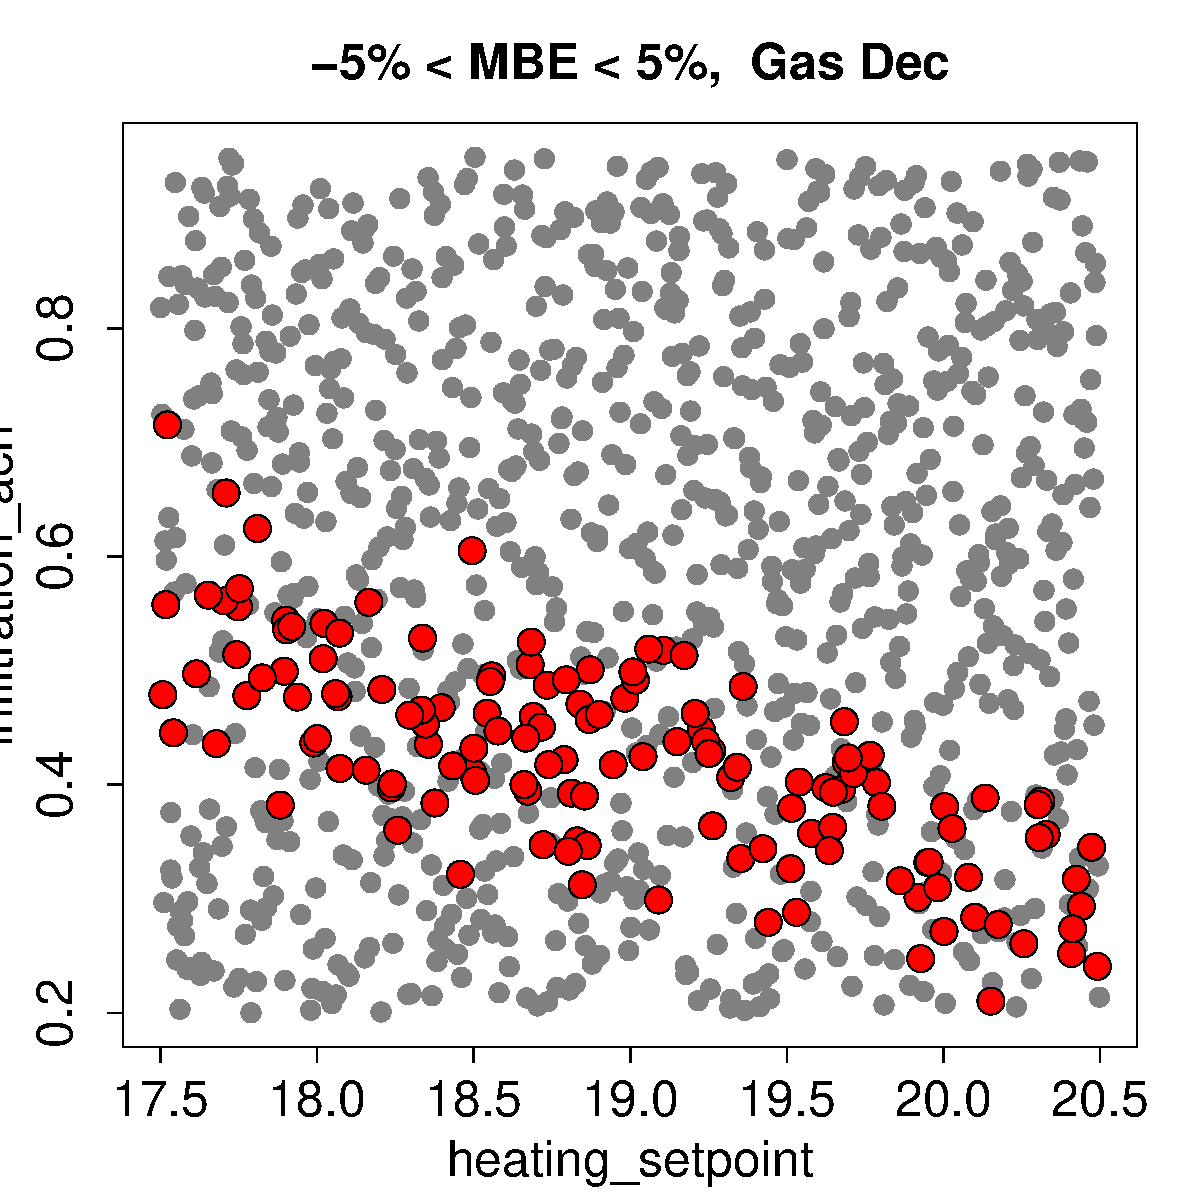
\includegraphics[width=\scale]{MBE/SelectedMBE_Gas_12.pdf}\\
 \caption{Scatter plots of the first (heating setpoint) and sixth (infiltration rate) coordinates of the 1000 simulations. In red, the points for which the Gas MBE satisfies $-5\% \leq \text{MBE} \leq 5\%$. None of the points satisfies the condition for any of the three summer months. Even besides the three months, there is, for example, no common red point between the plots of March and April.}
 \label{Fig_Output_Hist}
\end{figure}

%%%%%%%%%%%%%

















\end{document}


